% mnras_template.tex
%
% LaTeX template for creating an MNRAS paper
%
% v3.0 released 14 May 2015
% (version numbers match those of mnras.cls)
%
% Copyright (C) Royal Astronomical Society 2015
% Authors:
% Keith T. Smith (Royal Astronomical Society)

% Change log
%
% v3.0 May 2015
%    Renamed to match the new package name
%    Version number matches mnras.cls
%    A few minor tweaks to wording
% v1.0 September 2013
%    Beta testing only - never publicly released
%    First version: a simple (ish) template for creating an MNRAS paper

%%%%%%%%%%%%%%%%%%%%%%%%%%%%%%%%%%%%%%%%%%%%%%%%%%
% Basic setup. Most papers should leave these options alone.
\documentclass[a4paper,fleqn,usenatbib]{mnras}

% MNRAS is set in Times font. If you don't have this installed (most LaTeX
% installations will be fine) or prefer the old Computer Modern fonts, comment
% out the following line
\usepackage{newtxtext,newtxmath}
% Depending on your LaTeX fonts installation, you might get better results with one of these:
%\usepackage{mathptmx}
%\usepackage{txfonts}

% Use vector fonts, so it zooms properly in on-screen viewing software
% Don't change these lines unless you know what you are doing
\usepackage[T1]{fontenc}
\usepackage{ae,aecompl}


%%%%% AUTHORS - PLACE YOUR OWN PACKAGES HERE %%%%%

% Only include extra packages if you really need them. Common packages are:
\usepackage{graphicx}	% Including figure files
\usepackage{amsmath}	% Advanced maths commands
\usepackage{amssymb}	% Extra maths symbols

\usepackage{multirow}
\usepackage{lineno}
\linenumbers
%\usepackage{todonotes}

%%%%%%%%%%%%%%%%%%%%%%%%%%%%%%%%%%%%%%%%%%%%%%%%%%

%%%%% AUTHORS - PLACE YOUR OWN COMMANDS HERE %%%%%

% Please keep new commands to a minimum, and use \newcommand not \def to avoid
% overwriting existing commands. Example:
%\newcommand{\pcm}{\,cm$^{-2}$}	% per cm-squared

%%%%%%%%%%%%%%%%%%%%%%%%%%%%%%%%%%%%%%%%%%%%%%%%%%

%%%%%%%%%%%%%%%%%%% TITLE PAGE %%%%%%%%%%%%%%%%%%%

% Title of the paper, and the short title which is used in the headers.
% Keep the title short and informative.
\title[Short title, max. 45 characters]{Evaluation of data compression techniques for the inference of
  stellar atmospheric parameters from high resolution spectra}

% The list of authors, and the short list which is used in the headers.
% If you need two or more lines of authors, add an extra line using \newauthor
\author[K. T. Smith et al.]{
Keith T. Smith,$^{1}$\thanks{E-mail: mn@ras.org.uk (KTS)}
A. N. Other,$^{2}$
Third Author$^{2,3}$
and Fourth Author$^{3}$
\\
% List of institutions
$^{1}$Royal Astronomical Society, Burlington House, Piccadilly, London W1J 0BQ, UK\\
$^{2}$Department, Institution, Street Address, City Postal Code, Country\\
$^{3}$Another Department, Different Institution, Street Address, City Postal Code, Country
}

% These dates will be filled out by the publisher
\date{Accepted XXX. Received YYY; in original form ZZZ}

% Enter the current year, for the copyright statements etc.
\pubyear{2015}

% Don't change these lines
\begin{document}
\label{firstpage}
\pagerange{\pageref{firstpage}--\pageref{lastpage}}
\maketitle

% Abstract of the paper
\begin{abstract}
We evaluate the utility of several data compression techniques
  for alleviating the curse-of-dimensionality problem in regression
  tasks where the objective is to estimate stellar atmospheric
  parameters from high resolution spectra in the 4000-8000 K range. We
  conclude that ICA and kernel-PCA perform better than the rest of the
  techniques evaluated for all compression ratios. We also assess the
  necessity to adapt the signal-to-noise ratio (SNR) of the training
  set examples to the SNR of each test spectrum and conclude that
  within the conditions of our experiments, only two such models are
  needed (SNR=50 and 10) to cover the entire range.
\end{abstract}

% Select between one and six entries from the list of approved keywords.
% Don't make up new ones.
\begin{keywords}
Dimensionality Reduction -- keyword2 -- keyword3
\end{keywords}

%%%%%%%%%%%%%%%%%%%%%%%%%%%%%%%%%%%%%%%%%%%%%%%%%%

%%%%%%%%%%%%%%%%% BODY OF PAPER %%%%%%%%%%%%%%%%%%

\section{Introduction}

The rapid evolution of astronomical instrumentation and the
implementation of extensive surveys have permitted the acquisition of
vast amounts of spectral data.  The reduction and management of large
spectral databases collected by large-area or all-sky surveys like
Gaia/Gaia-ESO \citep{2006MNRAS.367..290J,2012Msngr.147...25G}, RAVE
\citep{2006AJ....132.1645S}, or APOGEE \citep{2011AJ....142...72E}
require the use of automatic techniques for the consistent,
homogeneous, and efficient extraction of physical properties from
spectra. The availability of these huge databases opens new
possibilities to better understand the stellar, Galactic, and
extra-galactic astrophysics. Of special importance is the
determination of intrinsic stellar physical properties, such as
effective temperature ($T_{\rm eff}$), surface gravity (log
\textit{g}), metallicity ([M/H]) and alpha to iron ratio 
($\left[ \alpha/Fe \right]$). However, the difficulty that
atmospheric parameter estimation poses comes from the inherent size
and dimensionality of the data.  Regression from stellar spectra
suffers the so-called {\sl curse of dimensionality} problem because
the number of variables (wavelengths) is much higher than the number
of training samples. 
    
The \textit{curse of dimensionality} \citep{bellman:61} relates to 
the problem caused by the exponential increase in volume associated 
with adding extra dimensions to Euclidean space. 
When the dimensionality increases, the volume of the space increases so 
fast that the available data become sparse. Because this sparsity is 
problematic for any method that requires statistical significance, the 
amount of data needed to support the result often grows exponentially 
with the dimensionality in order to obtain a statistically sound and 
reliable outcome.

Furthermore, typical spectra obtained in many surveys do not 
regularly reach the high signal-to-noise ratios (SNR) --about
100 or greater -- needed to obtain robust estimates, which
increases the difficulty to accurately estimate the physical
parameters of spectra.  In summary, stellar spectra are high
dimensional noisy vectors of real numbers and thus,
regression models must be both computationally efficient and robust
to noise.

There are several ways to alleviate this so-called \textit{curse of
  dimensionality}. It is evident that not all wavelength bins in an
observed spectrum carry the same amount of information about the
physical parameters of the stellar atmosphere. One way to reduce the
dimensionality of the space of independent variables is to concentrate
on certain wavelength ranges that contain spectral lines that are
sensitive to changes in the physical parameters. Before the
advent of the large-scale spectroscopic surveys, astronomers derived
physical parameters by interactively synthesizing spectra until a
subjective best fit of the observed spectrum in certain spectral lines
was found. But the number of spectra made available to the community
in the past decades have made this manual and subjective (thus
irreproducible) fitting procedure impractical. Automatic regression
techniques have therefore become a necessity.

The next step consisted in using derived features of the spectrum such
as fluxes, flux ratios or equivalent widths to infer the parameters
via multivariate regression techniques (see
\cite{2006ApJ...636..804A}, \cite{2012ApJ...750L..37M}, or
\cite{2006A&A...456.1109M}). That way, we significantly reduce the
full spectrum to a much smaller number of independent variables, at
the expense of introducing a feature extraction process: defining a
continuum level and normalizing the observed spectrum in the
wavelength region that contains the sensitive spectral feature. This
is potentially dangerous because, even in the best case that the
continuum flux is Gaussian distributed around a value significantly
different from zero, the ratio distribution is asymmetric and has a
heavy right tail. In the cases of low signal-to-noise spectra, the
situation can be catastrophic.

The potential dangers associated with the feature extraction in
restricted wavelength ranges via continuum normalisation can be
mitigated by projecting the observed spectra onto bases of functions
spaces such as in the wavelet or Fourier decompositions (see
\cite{2010PASP..122..608M}, \cite{2015MNRAS.452.1394L}, or
\cite{2015ApJS..218....3L} for examples of the two approaches).

In recent years, there seems to be a tendency to use the full spectrum
rather than selected wavelength ranges (see
e.g. \cite{2014A&A...567A...5R}, \cite{2015ApJ...808...16N},
\cite{2015MNRAS.448.2717W}, or \cite{2015arXiv151000111R}). In this
work we focus in this latter approach, and attempt to assess the
relative merits of various techiques to serve as a guide for future
applications of machine learning techiques for regression of stellar
atmospheric physical parameters.

The most popular dimensionality reduction technique applied to stellar
spectra is Principal Component Analysis (PCA). It has been widely
applied in spectral classification combined with artificial neural
networks (ANNs) \citep{singh:98} or support vector machines (SVM)
\citep{fiorentin:08b}. For continuum emission, PCA has a proven record
in representing the variation in the spectral properties of
galaxies. However, it does not perform well when reconstructing
high-frequency structure within a spectrum \citep{vanderplas:09}. To
overcome this difficulty, other methods have been used in the spectral
feature extraction procedure. Locally linear embedding (LLE)
\citep{roweisLLE:00} and Isometric feature map (Isomap)
\citep{tenenbaum:00} are two widely used nonlinear dimensionality
reduction techniques. Some studies found that LLE is efficient in
classifying galaxy spectra \citep{vanderplas:09} and stellar spectra
\citep{daniel:11}. Other authors concluded that Isomap performs better
than PCA, except on spectra with low SNR (between 5 and 10)
\citep{bu:14}.

A detailed study of data compression techniques has to include the
analysis of their stability properties against noise. In order to
improve the overall generalisation performance of the atmospheric
parameters estimators, experience shows that it is advantageous to
match the noise properties of the synthetic training sample to that of
the real sample because it acts as a regulariser in the training phase
\citep{fiorentin:08a}.  The impact of the SNR on the parameter
estimation ($T_{\rm eff}$, log \textit{g} and [Fe/H]) with artificial
neural networks (ANNs) is explored in \cite{snider:01}. They found
that reasonably accurate estimates can be obtained when networks are
trained with spectra --not derived parameters-- with similar SNR as
those of the unlabelled data, for ratios as low as 13.

\cite{recio:06} determined three atmospheric parameters
($T_{\rm eff}$, log \textit{g} and [M/H]) and individual chemical
abundances from stellar spectra using the MATISSE (MATrix
Inversion for Spectral SynthEsis) algorithm. They introduced Gaussian
white noise to yield five values of SNR between 25 and 200 and found
that errors increased considerably for SNR lower than $\sim$ 25.  In
\cite{navarro:12} authors present a system based on ANNs trained with
a set of line-strength indexes selected among the spectral lines more
sensitive to temperature and the best luminosity tracers. They
generated spectra with a range of SNR between 6 and 200 by adding
Poissonian noise to each spectrum. Their scheme allows to classify
spectra of SNR as low as 20 with an accuracy better than two spectral
subtypes. For SNR $\sim$ 10, classification is still possible but at a
lower precision.

This paper presents a comparative study of the most popular
dimensionality reduction technique applied to stellar spectra (PCA)
and five alternatives (two linear and three nonlinear techniques). The
aims of the paper are (1) to investigate to what extent novel
dimensionality reduction techniques outperform the traditional PCA on
stellar spectra datasets, (2) to test the robustness of these
techniques and their performance in atmospheric parameters estimation
for different SNRs, (3) to investigate the number of regression models
of different SNRs needed to obtain the best generalisation performance
for any reasonable SNR of the test data, and (4) to analyse the effect
of the grid density over the regression performance in atmospheric
parameters estimation.  The investigation is performed by an empirical
evaluation of the selected techniques on specifically designed
synthetic datasets. In Sect. \ref{sec:dimred} we review the data compression
techniques evaluated in this work and their properties. In
Sect. \ref{sec:dataset} we describe the dataset used in our experiments. 
Sect. \ref{sec:comparison1} presents our results when comparing the 
compression techniques and compression rates in terms of the atmospheric 
parameter estimation errors. In Sect. \ref{sec:comparison2} we evaluate 
the optimal match between the SNR of the training set examples to the SNR 
of the prediction test, and in Sect. \ref{sec:comparison3} we present 
the main results from the analysis of the effect of the training set grid 
density over the regression performance. Finally, in Sect. 
\ref{sec:conclusions} we summarize the most relevant findings from 
the experiments and discuss their validity and limitations.

\section{Dimensionality reduction}
\label{sec:dimred}

For the sake of computational efficiency in a dynamic environment
where a complete rerun of a dimensionality reduction algorithm becomes
prohibitively time consuming, the selection of the dimensionality
reduction techniques tested in our experiments was done amongst those
capable of projecting new data onto the reduced dimensional space
defined by the training set without having to re-apply the algorithm
(process also known as out-of-sample extension). Thus, in this work,
we investigated three linear dimensionality reduction techniques such
as PCA, independent component analysis (ICA) and discriminative
locality alignment (DLA), as well as three nonlinear reduction
techniques that do not lack generalisation to new data: wavelets,
Kernel PCA and diffusion maps (DM).  We aimed at minimizing the
regression error in estimating stellar atmospheric parameters with no
consideration of the physicality of the compression
coefficients. Physicality of the coefficients is sometimes required,
for example, when trying to interpret galactic spectra as a
combination of non-negative components.

Other linear and nonlinear techniques could be used for dimensionality
reduction, such as linear discriminant analysis (LDA), locally linear
embedding (LLE), Isomap, etc. When the number of variables is much
higher than that of training samples, classical LDA cannot be directly
applied because all scatter matrices are singular and this method
requires the non-singularity of the scatter matrices involved.
Isomap's performance exceeds the performance of LLE, specially when
the data is sparse. However, in presence of noise or when the data is
sparsely sampled, short-circuit edges pose a threat to both Isomaps
and LLE algorithms \citep{saxena:04}. Short-circuit edges can lead to
low-dimensional embeddings that do not preserve a manifold's true
topology \citep{balasubramanianISOMAP:02}. Furthermore, Isomap and LLE
cannot be extended out-of-sample. 

%\begin{itemize}
%\item PCA. Linear, unsupervised
%\item ICA. Linear, unsupervised
%\item DLA. Linear, supervised
%\item Diffusion Maps. Non-linear, preserving global properties
%\item Wavelets. Non-linear, preserving global properties
%\item Kernel PCA. Non-linear, preserving global properties
%\end{itemize}

\subsection{Principal Component Analysis (PCA)}

Principal Components Analysis (PCA) \citep{hotelling:33,pearson:01} is
by far the most popular (unsupervised) linear technique for
dimensionality reduction. The aim of the method is to reduce the
dimensionality of multivariate data whilst preserving as much of the
relevant information (assumed to be related to the variance in the
data) as possible. This is done by finding a linear basis of reduced
dimensionality for the data, in which the amount of variance in the
data is maximal. It is important to remark that PCA is based on the
assumption that variance is tantamount to relevance for the regression
task.

PCA transforms the original set of variables into a new set of
uncorrelated variables, the principal components, which are linear
combinations of the original variables. The new uncorrelated variables
are sorted in decreasing order of variance explained. The first
new variable shows the maximum amount of variance; the second
new variable contains the maximum amount of variation unexplained by
the first one, and is orthogonal to it, and so on.  This is
achieved by computing the covariance matrix for the full data
set. Next, the eigenvectors and eigenvalues of the covariance matrix
are computed, and sorted according to decreasing eigenvalue.

\subsection{Independent Component Analysis (ICA)}

Independent Component Analysis (ICA) \citep{comon:94} is very closely
related to the method called blind source separation (BSS) or blind
signal separation \citep{jutten:91}. It is the identification and
separation of mixtures of sources with little prior information. The
goal of the method is to find a linear representation of non-Gaussian
data so that the components are statistically independent, or as
independent as possible \citep{hyvarinen:00}.

Several algorithms have been developed for performing ICA
\citep{bell:95,belouchrani:97,ollila:06,li:08}. A large widely used
one is the FastICA algorithm \citep{hyvarinen:00} which has a number
of desirable properties, including fast convergence, global
convergence for kurtosis-based contrasts, and the lack of any step
size parameter.  RobustICA \citep{zarzoso:10} represents a simple
modification of FastICA, and is based on the normalised kurtosis
contrast function, which is optimised by a computationally efficient
iterative technique. It is more robust than FastICA and has a very
high convergence speed.  Another widely used ICA algorithm is the
Joint Approximation Diagonalisation of Eigen-matrices (JADE)
\citep{cardoso:93}. This approach exploits the fourth-order moments in
order to separate the source signals from mixed signals. In this work
we selected the JADE algorithm for projecting the original spectra in
the space of independent components.

\subsection{Discriminative Locality Alignment (DLA)}
Discriminative Locality Alignment (DLA) \citep{zhang:2008} is a
supervised manifold learning algorithm which can be divided into three
stages: part optimisation, sample weighting and whole alignment. In
the first stage, for each sample (each spectrum in our case) a patch
is defined by the given sample and its neighbours. On each patch, DLA
preserves the local discriminative information through integrating the
two criteria that {\textit{i}) the distances between intra-class
  samples are as small as possible and \textit{ii}) the distance
  between the inter-class samples is as large as possible. In the
  second stage, each part optimisation is weighted by the
  \textit{margin degree}, a measure of the importance of a given
  sample for classification. Finally, DLA integrates all the weighted
  part optimisations to form a global subspace structure through an
  alignment operation \citep{2002cs.......12008Z}. The projection
  matrix can be obtained by solving a standard eigendecomposition
  problem.

DLA requires the selection of the following two parameters:
\begin{itemize}
\item Neighbour samples from an identical class ($k_1$): 
	the number of nearest neighbours with respect to $x_i$
	from samples in the same class with $x_i$
\item Neighbour samples from different classes ($k_2$): 
	the number of nearest neighbours with respect to $x_i$
	from samples in different classes with $x_i$
\end{itemize}

This method obtains robust classification performance under the
condition of small sample size. Furthermore, it does not need to
compute the inverse of a matrix, and thus it does not face the matrix
singularity problem that makes linear discriminant analysis (LDA) and
quadratic discriminant analysis (QDA) not directly applicable to
stellar spectral data.

\subsection{Diffusion Maps}

Diffusion maps (DM) \citep{coifman:06,nadler:06} are a non linear
dimensionality reduction technique for finding the feature
representation of the datasets even if observed samples are
non-uniformly distributed.

DMs achieve dimensionality reduction by re-organizing data according
to parameters of its underlying geometry. DM are based on defining a
Markov random walk on the data. By performing the random walk for a
number of time steps, a measure for the proximity of the data points
is obtained (\textit{diffusion distance}). In the low-dimensional
representation of the data, DMs attempt to retain the pairwise
diffusion distances as faithfully as possible (under a squared error
criterion). The key idea behind the diffusion distance is that it is
based on integrating over all paths through the graph. This makes the
diffusion distance more robust to short-circuiting than, e.g., the
geodesic distance that is employed in Isomap \citep{tenenbaum:00}.

In this work, the results were optimised by controlling the degree of
locality in the diffusion weight matrix (parameter \textit{eps.val}).

\subsection{Wavelets}

Wavelets \citep{mallat:98} are a set of mathematical functions used to
approximate data and more complex functions by decomposing the signal
in a hybrid space that incorporates both the original space where the
data lie (which we will refer to as original space), and the
transformed frequency domain. In our case, the original space will be
the wavelength space, but in representing time series with wavelets
the original space would be the time axis. The wavelet transform is a
popular feature definition technique that has been developed to
improve the shortcomings of the Fourier transform. Wavelets are
considered better than Fourier analysis for modelling because they
maintain the original space information while including information
from the frequency domain.

Wavelets can be constructed from a function (named \textit{mother
  wavelet}), which is confined to a finite interval in the original
space. This function is used to generate a set of functions through
the operation of scaling and dilation applied to the mother
wavelet. The orthogonal or biorthogonal bases formed by this set
allows the decomposition of any given signal using inner products,
like in Fourier analysis. This method offers multi-resolution analysis
in the original space and its frequency transformed domain, and it can
be useful to reveal trends, breakdown points or discontinuities.

Dimensionality reduction with wavelets consists of keeping a reduced
number of wavelet coefficients. There are two common ways of
coefficient selection: ({\textit i) to eliminate the high frequency
  coefficients that are assumed to reflect only random noise, and
  ({\textit ii) to keep the $k$ most statistically significant
    coefficients (which yields a representation of the signal with
    less variance) \citep{li:10}. There are more sophisticated ways to
    further reduce the number of coefficients using standard machine
    learning techniques for feature selection, such as the LASSO
    (Least Absolute Shrinkage and Selection Operator) used in
    \cite{2015MNRAS.452.1394L}, wrapper approaches, information theory
    measures, etc. A full analysis of all these alternatives is out of
    the scope of this paper and we will only apply the first reduction
    mentioned above.

\subsection{Kernel PCA}

Kernel PCA (KPCA) is the reformulation of traditional linear PCA in a
high-dimensional space that is constructed using a kernel function
\citep{sholkopf:98}. This method computes the principal eigenvectors
of the kernel matrix, rather than those of the covariance matrix. The
reformulation of PCA in kernel space is straightforward, since a
kernel matrix is similar to the inner product of the datapoints in the
high-dimensional space that is constructed using the kernel function
(the so-called {\textit kernel trick}). The application of PCA in the
kernel space allows for the construction of nonlinear mappings of the
input space.

Since Kernel PCA is a kernel-based method, the mapping performed
relies on the choice of the kernel function. Possible choices for the
kernel function include the linear kernel (i.e., traditional PCA), the
polynomial kernel, and the Gaussian kernel. An important weakness of
Kernel PCA is that the size of the kernel matrix is proportional to
the square of the number of instances in the dataset.

In this work we used the Gaussian kernel and optimized the predictive
performance by fine tuning the inverse kernel width ($\sigma$).
 
\section{The dataset}
\label{sec:dataset}
The synthetic spectra that form the basis of our study have been
computed from MARCS model atmospheres \citep{gustafsson:08} and the
turbospectrum code \citep{alvarez:98, plez:12} together with atomic \&
molecular line lists. These spectra were kindly provided by the
Gaia-ESO team in charge of producing the physical parameters for the
survey.

The datasets used in this work contain a grid of 8780 synthetic 
high-resolution spectra with effective temperatures between 4000 and 
8000 K (step 250 K), logarithmic surface gravities between 1.0 and 5.0 
(step 0.5), mean metallicities between -3.0 and 1.0 (with a variable step 
of 0.5 or 0.25 dex) and $\left[ \alpha/Fe \right]$ values varying between
-0.4 and +0.4 dex (step 0.2 dex) around the standard relation with the
following $\alpha$ enhancements: $\left[ \alpha/Fe \right]$ = +0.0 dex
for [M/H] $\geqslant$ 0, $\left[ \alpha/Fe \right]$ = +0.4 dex for
[M/H] = $\leqslant$ -1.0 and $\left[ \alpha/Fe \right]$ = -0.4[M/H]
for [M/H] between -1.0 and +0.0 (Fig.~\ref{fig:gridModelos}).
Elements considered to be $\alpha$-elements are O, Ne, Mg, Si, S, Ar,
Ca and Ti. The adopted solar abundances are those used by
\citep{gustafsson:08}.  

\begin{figure}
\centering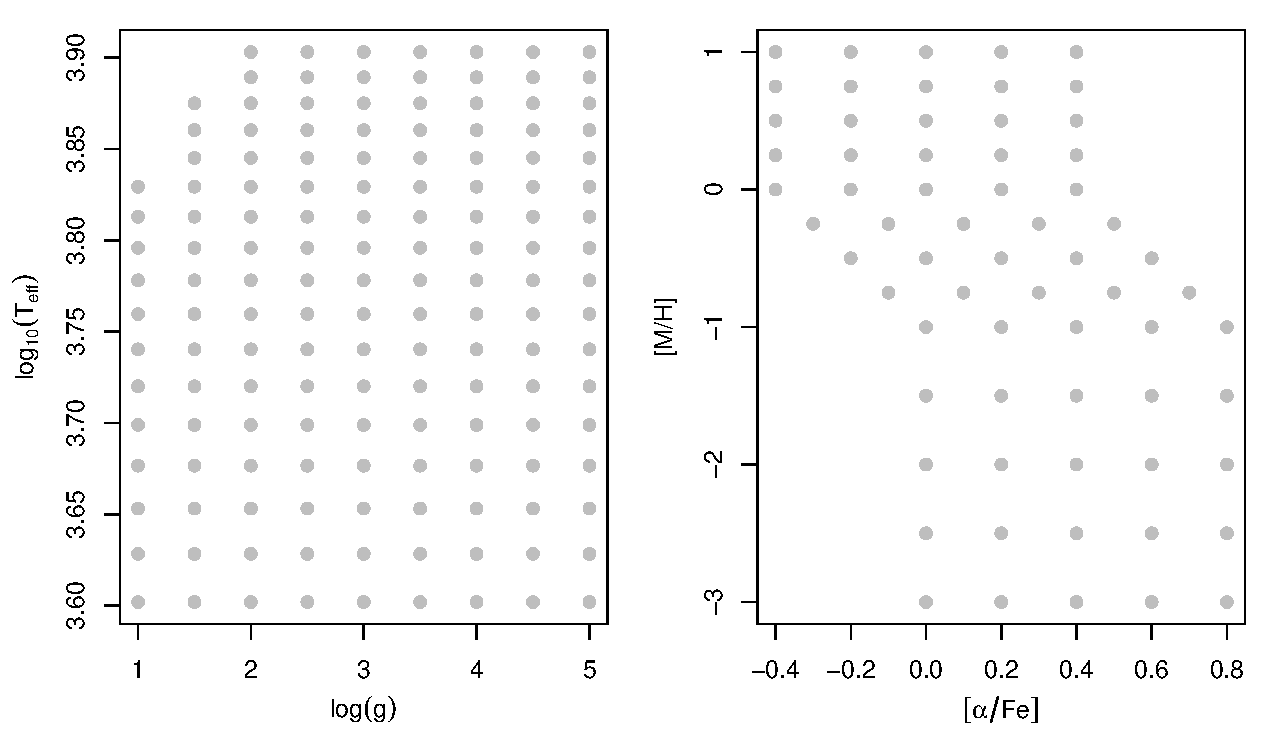
\includegraphics[width=\columnwidth]{grid_modelos.pdf}
\caption{Coverage in parameter space of the dataset}
\label{fig:gridModelos}
\end{figure}

More specifically, we used two datasets covering two ranges in 
wavelength: (1) a dataset containing high-resolution spectra 
(\textit{R} = 19800) between 5339 and 5619 {\AA} (the nominal GIRAFFE 
HR10 setup) and (2) a dataset containing high-resolution spectra
(\textit{R} = 16200) between 8484 and 9001 {\AA} (the nominal GIRAFFE 
HR21 setup). Fig.~\ref{fig:ejemplosEspectros} shows some
example spectra from this dataset.

%For each selected setup, the grid of spectra span the parameter ranges
%[4000, 8000] K in effective temperature (step 250 K), 
%[1.0, 5.0] in logarithmic surface gravities (step 0.5), 
%[-3.0, 1.0] in mean metallicities (with a variable step of 0.5
%or 0.25 dex), and 
%[-0.4, 0.4] dex in $\left[ \alpha/Fe \right]$ (step 0.2 dex). 

\begin{figure*}
\centering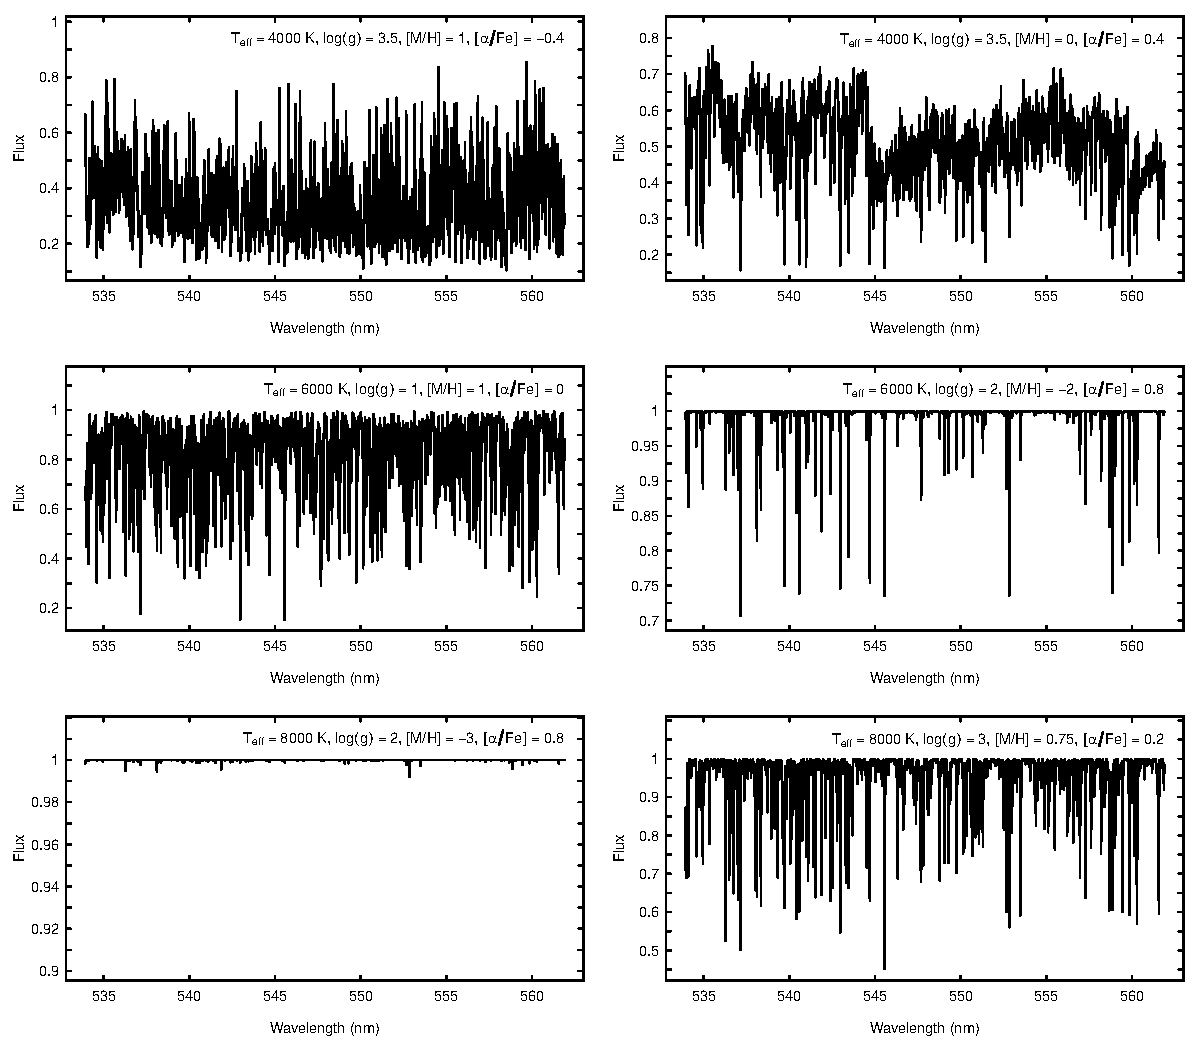
\includegraphics[width=\textwidth]{espectros01.pdf}
\caption{Example spectra from the first dataset (the nominal GIRAFFE 
HR10 setup).}
\label{fig:ejemplosEspectros}
\end{figure*}

\begin{figure*}
\centering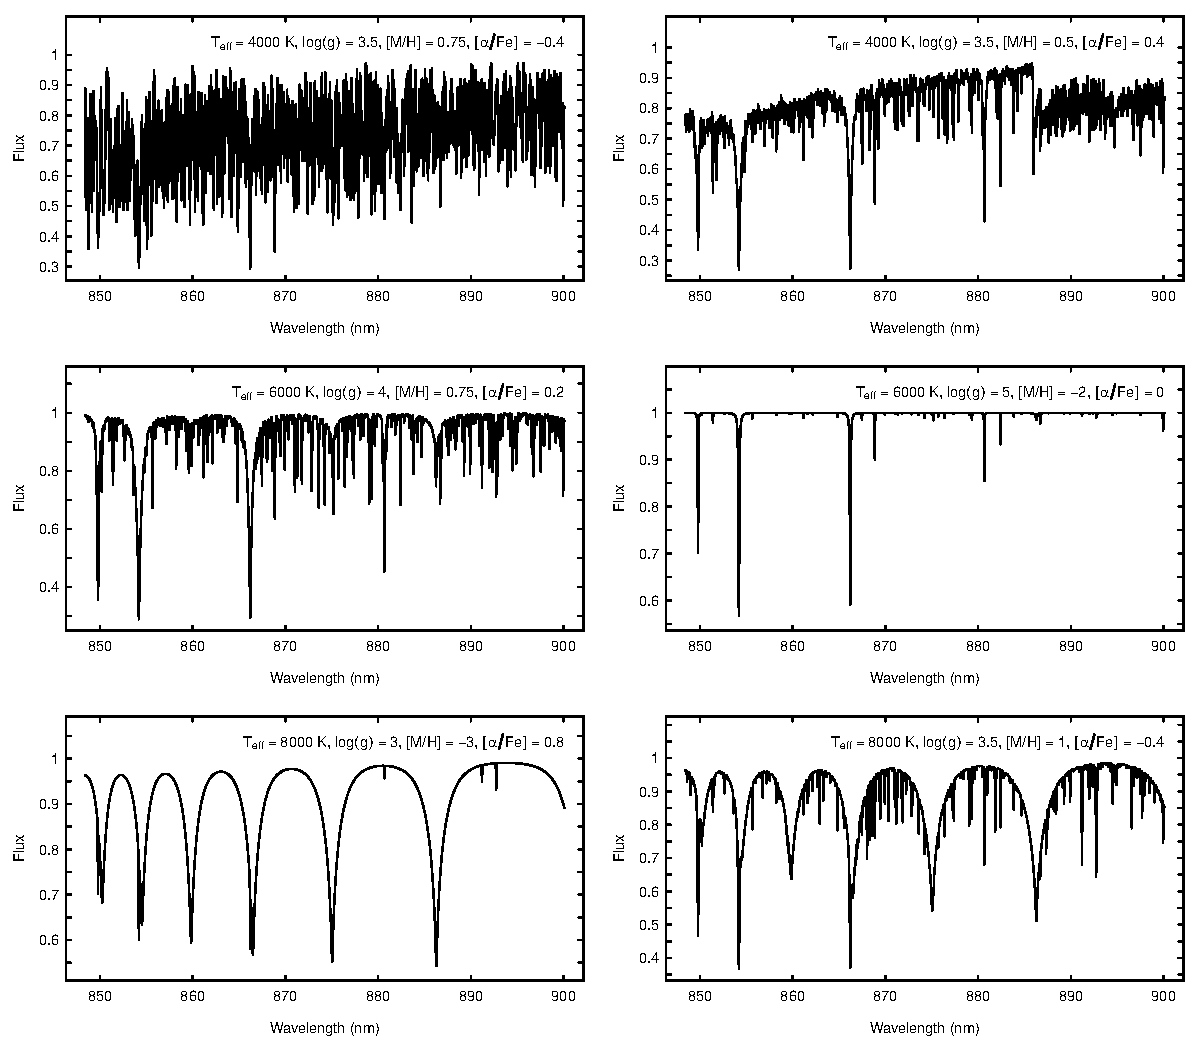
\includegraphics[width=\textwidth]{espectros02.pdf}
\caption{Example spectra from the second dataset (the nominal GIRAFFE 
HR21 setup).}
\label{fig:ejemplosEspectros}
\end{figure*}


The sample size of our datasets (8780 spectra) is relatively
small compared to the input dimension (2798 and 5168 flux 
measurements per spectrum, respectively). For example, with an 
amount of information about 10 samples per dimension --a rule of 
thumb is to have at least 10 training samples per feature dimension 
\citep{jain:00}, the dataset should contain $10^{2798}$ and 
$10^{5168}$ spectra, respectively.
In most real case applications, the ratio of sample size to input 
dimensions is much lower and thus, the \textit{curse of dimensionality} 
problem is expected to affect even more severely the inference process. 

The conclusions drawn from the set of experiments described below
depend on the restricted range of physical parameters, wavelengths,
and spectral resolution adopted in the dataset, but we hope that they
still hold for datasets of similar characteristics (different
wavelength ranges but similar resolutions and parameter subspaces). In
completely different scenarios such as the reddest regions of the
Hertzsprung-Russell diagram, where spectra are dominated by molecular
absoption bands, our results cannot be expected to apply in general.

\section{Comparison of spectrum compression techniques and optimal rates}
\label{sec:comparison1}

We investigate the utility of six dimensionality reduction techniques
for feature extraction with a view to improving the performance of
atmospheric parameters regression models. The robustness of these
techniques against increasing SNR is evaluated, and the generalisation
performance of training sets of varying SNRs is analysed.

Our set of experiments proceeds in three stages. In the first stage we
aim at comparing the various compression techniques and compression
rates in terms of the atmospheric parameter estimation errors. As a
result of these experiments, we select an optimal compression approach
and rate (dimensionality of the reduced space).

Different machine learning models have been used for the automatic
estimation of atmospheric parameters from stellar spectra. Two of the
most widely used techniques in practice are artificial neural networks
(ANN) and support vector machines (SVM). Unlike ANN, SVM does not need
a choice of architecture before training, but there are some
parameters to adjust in the kernel functions of the SVM. We use SVMs
with radial basis kernel functions and adjust the SVM parameters by
maximizing the quality of the atmospheric parameter ($T_{\rm eff}$,
log \textit{g}, [M/H] or $\left[ \alpha/Fe \right]$) prediction as 
measured by the root mean squared error (RMSE) (equation~(\ref{eq:rmse})) 
in out-of-sample validation experiments.

\begin{equation}
\label{eq:rmse}
RMSE=\sqrt{\frac{1}{n}\sum_{i=1}^{n}\left(\hat{T}_{i}-T_{i}\right)^{2}}
\end{equation}

where $\hat{T}_{i}$ is the predicted atmospheric parameter ($T_{\rm eff}$, 
  log \textit{g}, [M/H] or $\left[ \alpha/Fe \right]$) and 
  $T_{i}$ is the target value. 
  
The datasets were randomly split into two subsets, one for training
(66\% of the available spectra) and one for evaluation (the remaining
34\%). Since the goal of these first experiments is to compare the
reduction techniques rather than obtaining the best predictor,
splitting the dataset into training and evaluation sets is considered
a good scheme. In essence, the experimental procedure consists of the
following steps (Fig.~ \ref{fig:flowchart}):

\begin{enumerate}
\item \label{itemone} Compute the low-dimensional representation of
  the data using the training set. Because some of the techniques used
  to reduce the dimensionality depend on the setting of one or more
  parameters, a tuning process was performed in order to determine the
  optimal parameter values. Table~\ref{tab:parameters} presents the
  values that were evaluated, as well as the best parameter value
  obtained in each case.
\item \label{itemtwo} Construct SVM models using the training set, and a varying
  number of dimensions (2, 5, 10, 15, 20, 25, 30 and 40) of the
  reduced space. The SVM parameters (kernel size and soft-margin
  width) are fine-tuned to minimize the prediction error of the
  atmospheric parameter ($T_{\rm eff}$, log \textit{g}, [M/H] or 
  $\left[ \alpha/Fe \right]$).
\item \label{itemthree} Project the evaluation spectra onto the
  low-dimensional space computed in step \ref{itemone}.
\item Obtain atmospheric parameter estimations by applying the SVM
  models trained in step \ref{itemtwo} to the test cases obtained in
  step \ref{itemthree}.
\item Calculate the performance of the predictor based on the RMSE
  obtained on the evaluation set.
\end{enumerate}

\begin{figure*}
\centering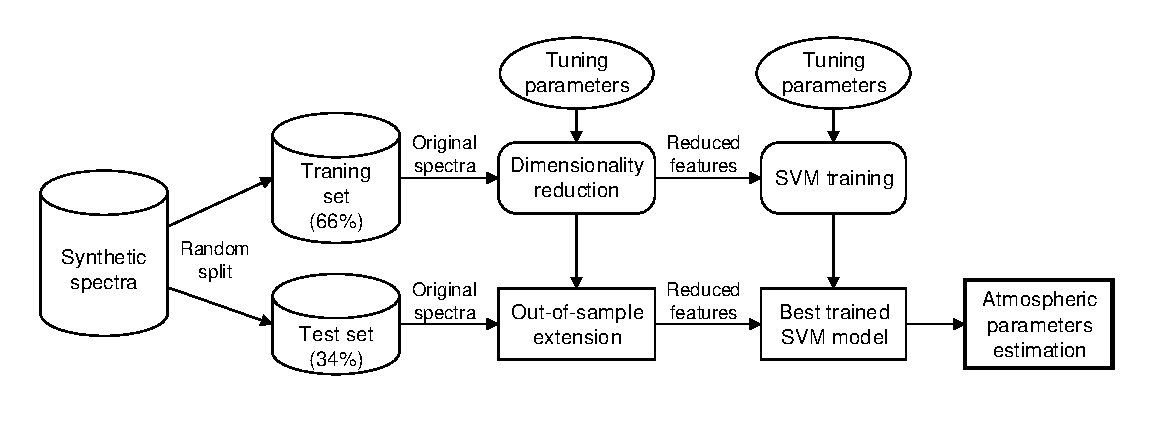
\includegraphics[width=0.8\textwidth]{flowchart.pdf}
\caption{Process flow chart for investigating the performance of the 
selected dimensionality reduction techniques.}
\label{fig:flowchart}
\end{figure*}

\begin{table}
\centering
\caption{Summary of the parameters analysed for the 
dimensionality reduction techniques.}
\label{tab:parameters}
\begin{tabular}{l c c c}
\hline
\textbf{Technique} & \textbf{Parameter} & \textbf{analysed range} & \textbf{Best value} \\
\hline
\multirow{2}{*}{DLA} 
	& $k_1$ & [2 - 8]  & 2 \\\cline{2-4}
	& $k_2$ & [2 - 8]  & 3 \\\hline
DMAP & eps.val & [0.01 - 700] & 600 \\\hline
KPCA & $\sigma$ & [0.0001 - 0.01] & 0.001 \\
\hline
\end{tabular}
\end{table}

The procedure described above is repeated for different SNR regimes in
order to study the dependency of the estimation performace on the
noise level of the input spectra. Gaussian white noise of different
variances (SNRs equal to 100, 50, 25 and 10) was added to the original
synthetic spectra. 

\subsection{Results}

First, we compare the performance of the dimensionality reduction
techniques described in section \ref{sec:dimred} using noise-free
synthetic spectra as well as degraded spectra with SNR levels of 100,
50, 25 and 10.  Figures \ref{fig:02} to \ref{fig:07} show the RMSE
obtained with the evaluation set (the 34\% of the full set of spectra
that was not not used to define the compression transformation or to
train SVM models).

\begin{figure*}
\centering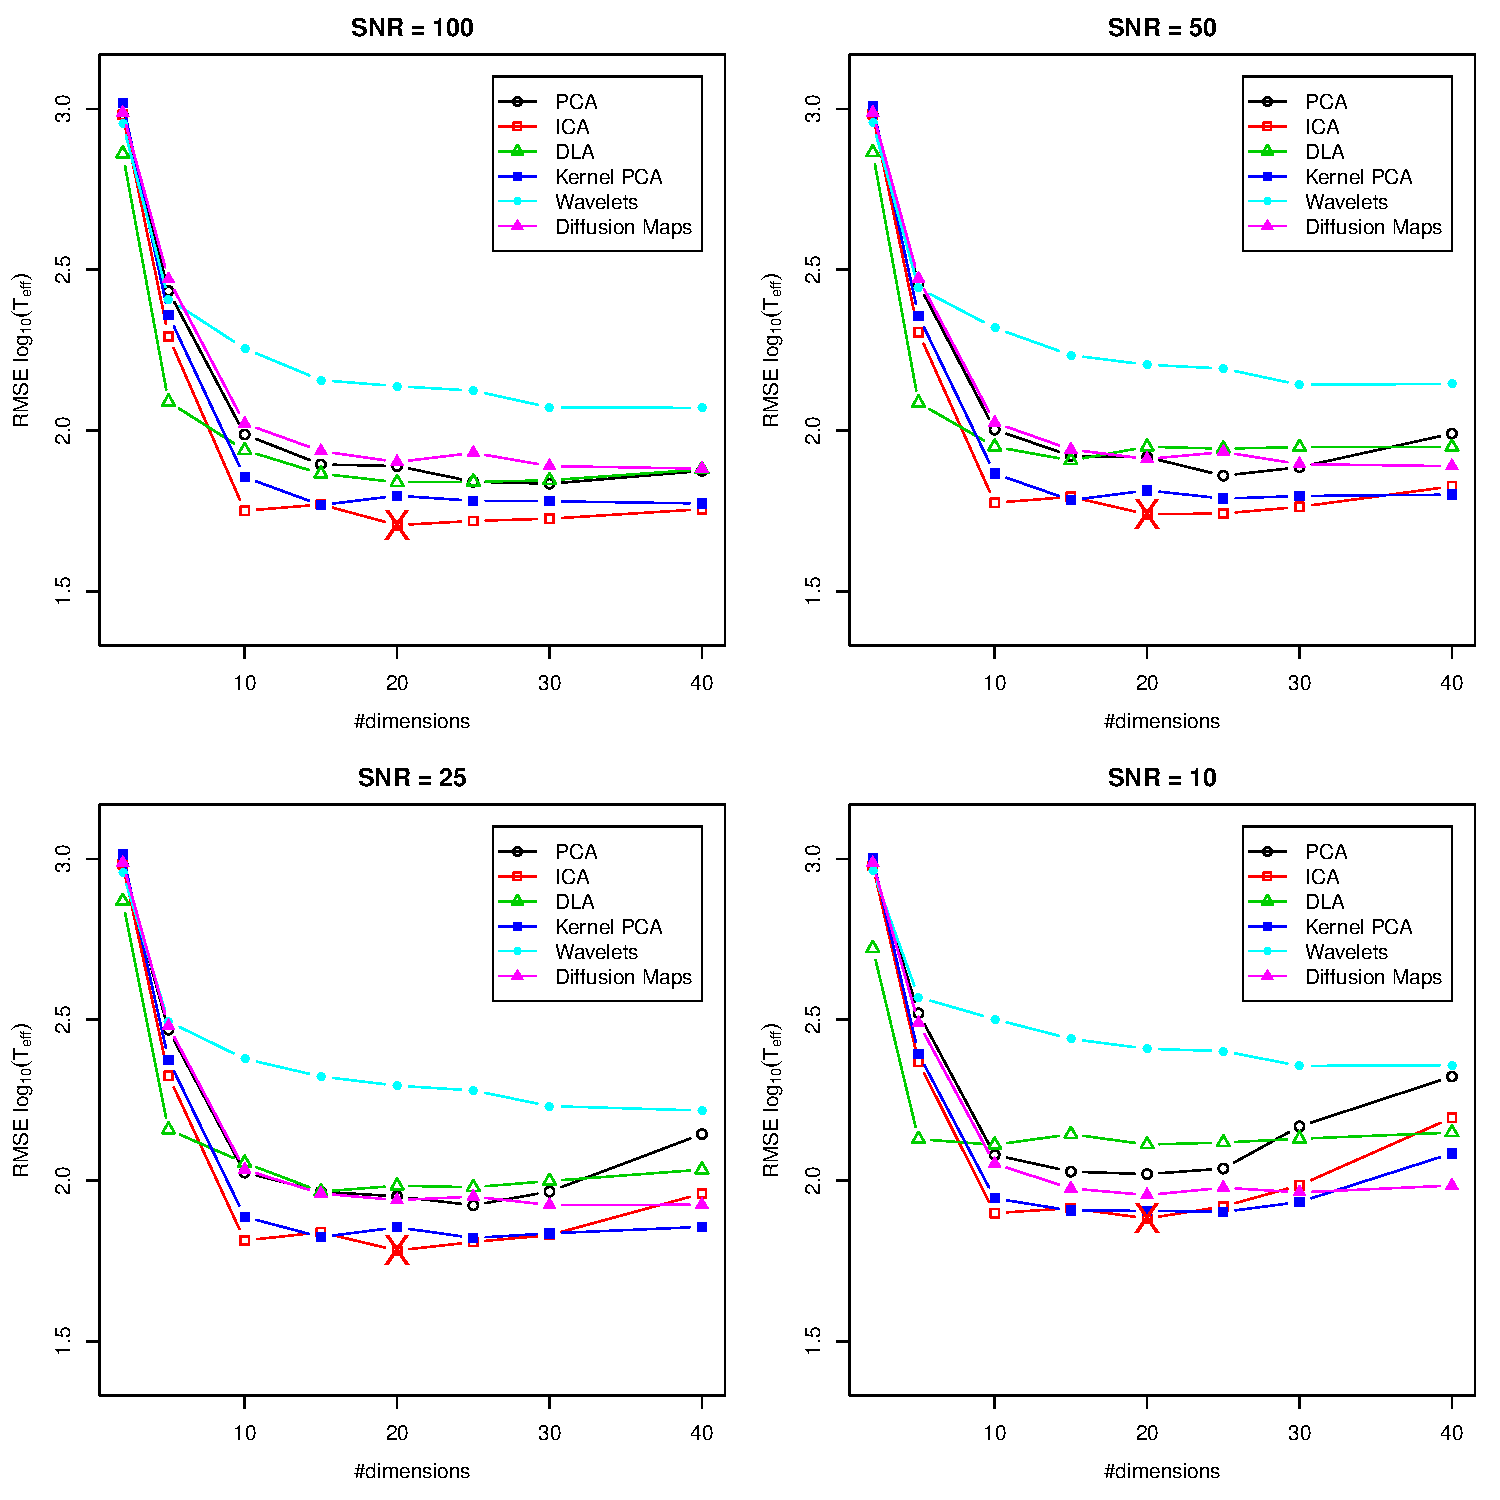
\includegraphics[width=\textwidth]{flamesHR10_Teff_log_BestSVM_N-RMSE_test.pdf}
\caption{Temperature estimation errors as a function of the number of
  dimensions used for data compression, for noisy synthetic
  spectra.}
\label{fig:02}
\end{figure*}

\begin{figure*}
\centering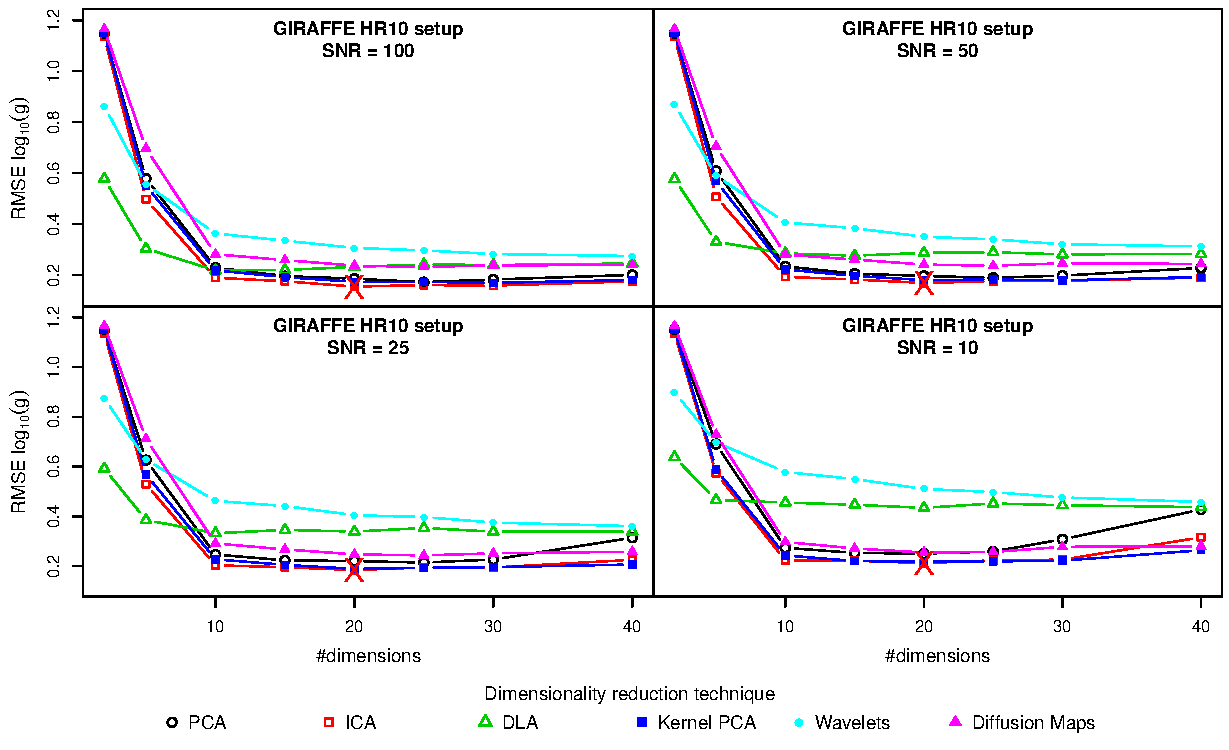
\includegraphics[width=\textwidth]{flamesHR10_Logg_BestSVM_N-RMSE_test.pdf}
\caption{Surface gravity estimation errors as a function of the number of
  dimensions used for data compression, for noisy synthetic
  spectra.}
\label{fig:04}
\end{figure*}

\begin{figure*}
\centering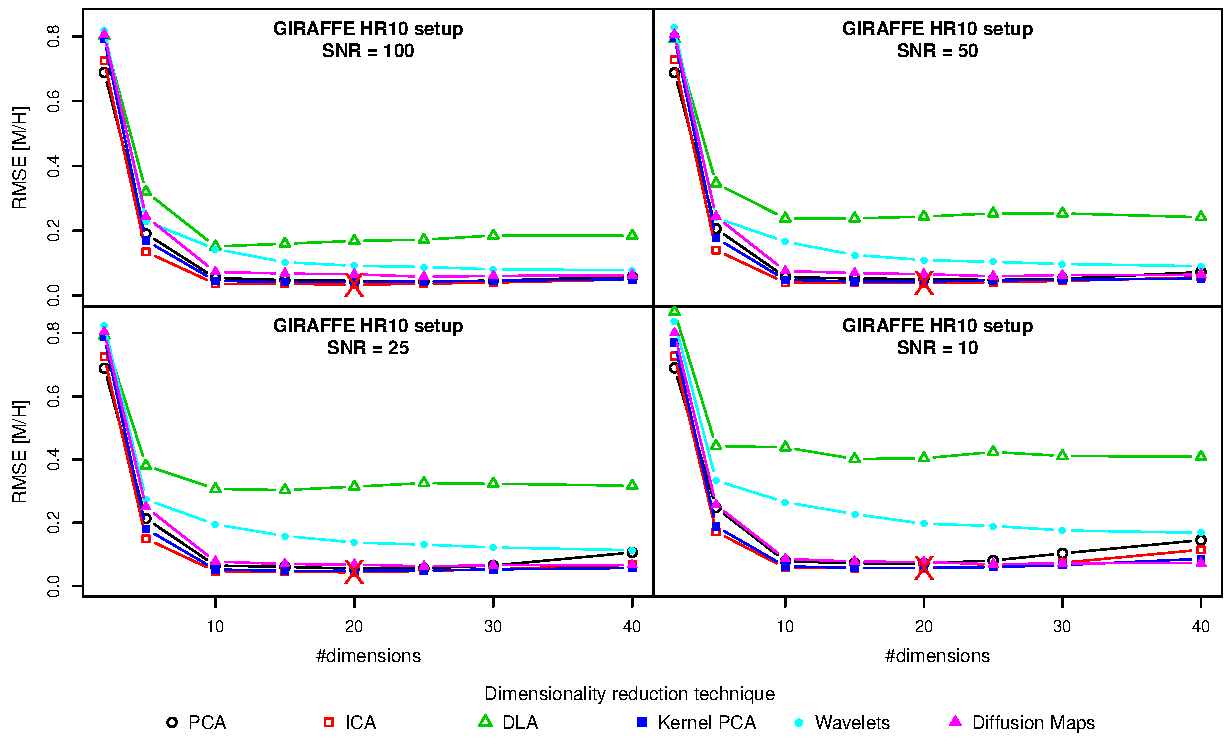
\includegraphics[width=\textwidth]{flamesHR10_Meta_BestSVM_N-RMSE_test.pdf}
\caption{Metallicity estimation errors as a function of the number of
  dimensions used for data compression, for noisy synthetic
  spectra.}
\label{fig:06}
\end{figure*}

\begin{figure*}
\centering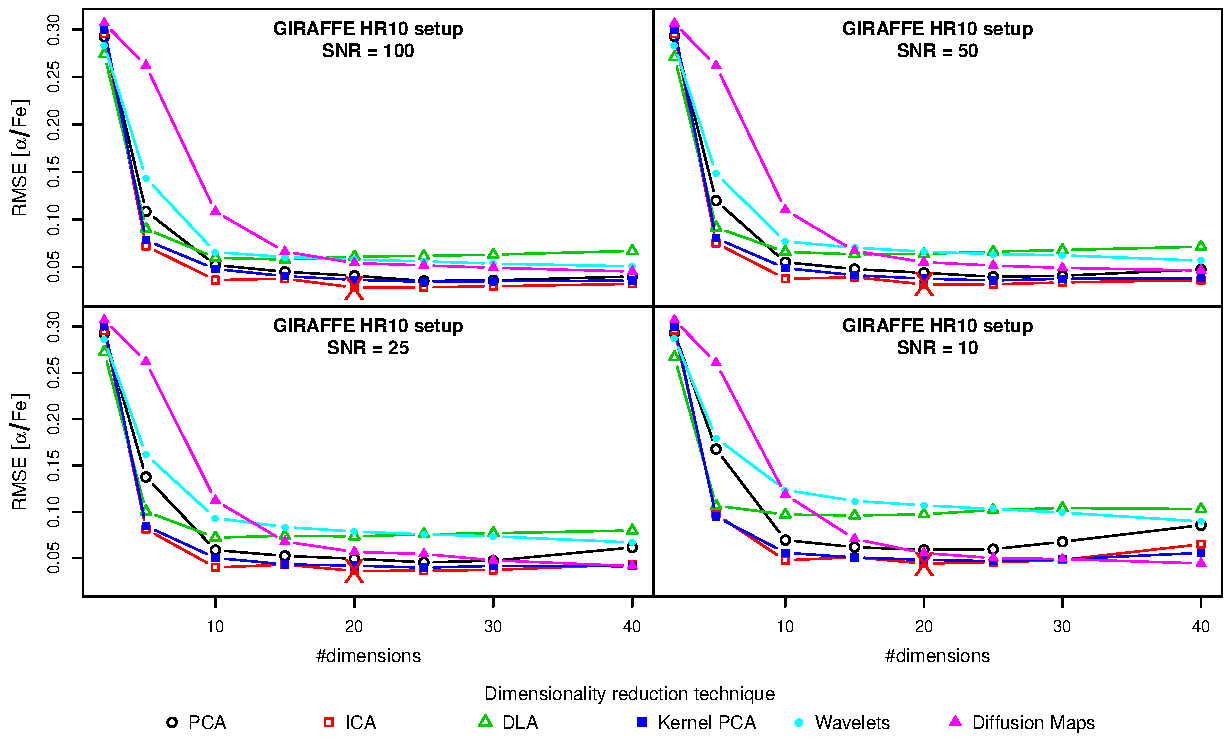
\includegraphics[width=\textwidth]{flamesHR10_AlFe_BestSVM_N-RMSE_test.pdf}
\caption{$\left[ \alpha/Fe \right]$  estimation errors as a function of the number of
  dimensions used for data compression, for noisy synthetic
  spectra.}
\label{fig:07}
\end{figure*}

Inspection of the figures reveals that the best strategies to compress
the spectra are kernel PCA and ICA, with ICA outperforming kernel PCA
in most of the parameter space, except sometimes for the lowest
compression rate. RMSE errors increase only moderately down to a SNR
of 10, which seems to indicate that most of the examined compression
techniques serve well as noise filters.

The performance comparison of the analysed dimensionality reduction
techniques shows that although traditional PCA is not the most
efficient method, it outperforms some of the nonlinear techniques used
in this study, such as diffusion maps or wavelets. {\bf We need
  to propose an explanation}. 

Overall, wavelets combined with SVM models have the highest errors
regardless of the number of retained dimensions, with the exception of
the [M/H] estimation where DLA performed worse for noisy synthetic
spectra. DLA achieved the lowest prediction errors for the unrealistic
noise-free data (not shown here for the sake of
conciseness). Furthermore, this technique yields the best performance
for the highest compression rates (two or five dimensions) when
estimating $T_{\rm eff}$ and log \textit{g}. However, it was
outperformed by most other techniques for almost any other compression
rate. PCA and diffusion maps yield similar $T_{\rm eff}$ prediction
errors in the high SNR regime, but DMs is more robust against noise
specially for the lowest compression rates examined.

It is interesting to note that compression techniques can be grouped
into two categories: DLA, DM and Wavelets show a flat RMSE for target
dimensions greater than ten, even for the lowest SNR explored in this
Section (SNR=10); PCA, Kernel PCA and ICA show positive slopes in the
RMSE curves for SNRs below 25 and target dimensionalities greater than
25, indicating that components beyond this limit are increasingly
sensitive to noise. 

The relative merit of Diffusion Maps with respect to the best
performing compression techniques (ICA and kernel PCA) improves as the
SNR diminishes until it becomes almost comparable for SNR=10, while at
the same time rendering the SVM regression module insensitive to the
introduction of irrelevant features (as shown by the flat RMSE curves
for increasing numbers of dimensions used). 

Table~\ref{tab:01} quantifies the prediction errors of the best models
for each SNR. It is interesting that ICA compression with 20
independent components remains as the best option for any SNR, except
for the unrealistic noise-free data (shown in Fig.~\ref{fig:01} in
Appendix~\ref{app}). These results evidence that for a given sample
size (the number of spectra in this particular application) there is
an optimal number of features beyond which the performance of the
predictor will degrade rather than improve.  On the other hand, as
expected, the quality of atmospheric parameter ($T_{\rm eff}$, log
\textit{g} or [M/H]) predictions degrades for lower SNR. However, RMSE
errors were relatively low even for low SNR ($\sim$ 10).  

\begin{table*}
\centering
\caption{RMSE on the evaluation set of 2986 spectra for the best SVM trained models.}
\label{tab:01}
%\resizebox{0.99\textwidth}{!}{%
\begin{tabular}{l c c c c c c}
\hline
\multirow{2}{*}{\textbf{SNR}} & \multirow{2}{*}{\textbf{Method}} & \multirow{2}{*}{\textbf{Nr. Dim.}} & {\bf RMSE} & {\bf RMSE} & {\bf RMSE} & {\bf RMSE}\\
 &  &  & \textbf{$T_{\rm eff}$ (K)} & \textbf{log \textit{g}} & \textbf{[M/H] (dex)}  & \textbf{$\left[ \alpha/Fe \right]$ (dex)}\\
\hline
$\infty$ & DLA / ICA\protect\footnotemark[1] & 40 / 30 / 20\protect\footnotemark[2] & 27.16 & 0.13 & 0.017 & 0.025\\
100 & ICA & 20 & 50.81 & 0.15 & 0.033 & 0.028\\
50 & ICA & 20 & 54.91 & 0.17 & 0.038 & 0.032\\
25 & ICA & 20 & 60.59 & 0.18 & 0.043 & 0.036\\
10 & ICA & 20 & 76.21 & 0.21 & 0.057 & 0.044\\
\hline
%\multicolumn{6}{l}{$^1$ }\\
\end{tabular}
%}
\end{table*}
\footnotetext[1]{The best performance for $T_{\rm eff}$, log
  \textit{g} and [M/H] was obtained with DLA, while best 
  performance for $\left[ \alpha/Fe \right]$ was obtained with ICA.}
\footnotetext[2]{The best performance for $T_{\rm eff}$ and log
  \textit{g} was obtained with 40 dimensions, while for [M/H] and 
  $\left[ \alpha/Fe \right]$, 30 and 20 dimensions were needed,
  respectively.}

%%%%%%%%%%%%%%%%%%%%%%%%%%%%%%%%%%%%%%%
\section{Optimal training set SNR}
\label{sec:comparison2}

In the second stage, we study the optimal match between the training
set SNR and that of the spectra for which the atmospheric parameter
predictions are needed (in the following, the prediction set).

In order to analyse the dependence of the predicition accuracy with
the training set SNR, we generate 25 realisations of the noise for
each of the following 8 finite SNR levels: 150, 125, 100, 75, 50, 25,
10 and 5. This amounts to $25\times 8=200$ datasets, plus the
noiseless dataset. We create the 25 noise realisation to estimate the
variance of the results. For each of these datasets we trained an SVM
model to estimate each of the atmospheric parameters ($T_{\rm
  eff}$, log \textit{g} or [M/H]), and to assess the consistency of
the results as the test set SNR degrades. The model performances were
evaluated using 10-fold cross validation as follows:

\begin{enumerate}
\item The noiseless dataset is replicated $25\times 8$ times: 25
  realisations of Gaussian white noise for each of the following SNRs:
  150, 125, 100, 75, 50, 25, 10, and 5. These 200 replicates together
  with the original noiseless dataset forms the basis for the next
  steps.
\item Each spectrum in each dataset is projected onto 20 independent
  components (as suggested by the experiments described in
  Section~\ref{sec:comparison1}).
\item Each of the 201 compressed datasets is then split into 10
  subsets or \textit{folds}. The splitting is unique for the 201
  datasets, which means that each spectrum belongs to the same fold
  across all 201 datasets.
\item \label{itemthree2} An SVM model is trained using 9 folds of each
  dataset (all characterized by the same SNR). This amounts to 201
  models.
\item \label{itemfour2} The model constructed in step \ref{itemthree2}
  is used to predict physical parameters for the tenth fold in all its
  201 versions. The RMSE is calculated independently for each value of
  the SNR and noise realisation.
\item \label{itemfive2} Steps \ref{itemthree2} to \ref{itemfour2} are
  repeated 10 times (using each time a different fold for evaluation)
  and the performance measure is calculated by averaging the values
  obtained in the loop.
\end{enumerate}

\subsection{Results}

Fig.~ \ref{fig:snrtrain} shows the mean (averaged over the 25 noise
realisations) RMSE results and the 95\% confidence interval for the
mean as a function of the SNR of the evaluation set. The nine
different lines correspond to the SNR of the training set used to
generate both the projector and the atmospheric parameters predictor.
The main conclusions of the analysis can be summarised as follows:

\begin{itemize}
\item This analysis yields the very important consequence that models
  trained with noise-free spectra are not adequate to estimate
  atmospheric parameters of spectra with SNRs up 50/75, and are
  unnecessary for $T_{\rm eff}$, log \textit{g} and $\left[ \alpha/Fe 
  \right]$ in contexts of even higher SNRs. Only the [M/H] regression 
  models slightly benefit from training with noiseless spectra if the test 
  spectra are in the SNR$\ge 50$ regime. The accuracy of the model 
  trained with noise-free spectra degrades exponentially for SNR$<$50.
\item There are no large discrepancies amongst the estimations
  obtained by applying the 25 models trained with a given SNR to
  different noise realisations, which translates into small confidence
  intervals and error bars in the plot. This is so even for the lowest
  SNR tested (SNR=5).
\item Only one ICA+SVM model trained with SNR of 25 would be enough to
  estimate the surface gravity for spectra of all SNRs with the best
  performance.
\item Only one ICA+SVM model trained with SNR of 50 would be enough to
  estimate the alpha to iron ratio for spectra of all SNRs with 
  the best performance.
\item For evaluation spectra with SNR$\ge 100$, there are minimal
  differences in the precision achieved by models trained with spectra
  of SNR$\ge 50$.  
\item For evaluation sets with $100\ge SNR > 10$, the best accuracy is
  obtained with the model constructed from spectra with SNR of 50
  (except in the case of log {\it g}, where the SNR=25 training set
  outperforms SNR=50 as noted above, but the difference is small).
\item For SNR lower than 10, the model with best generalisation
  performance is that trained with SNR equal to 10 for $T_{\rm eff}$ 
  and [M/H]. 
\end{itemize}

\begin{figure*}
\centering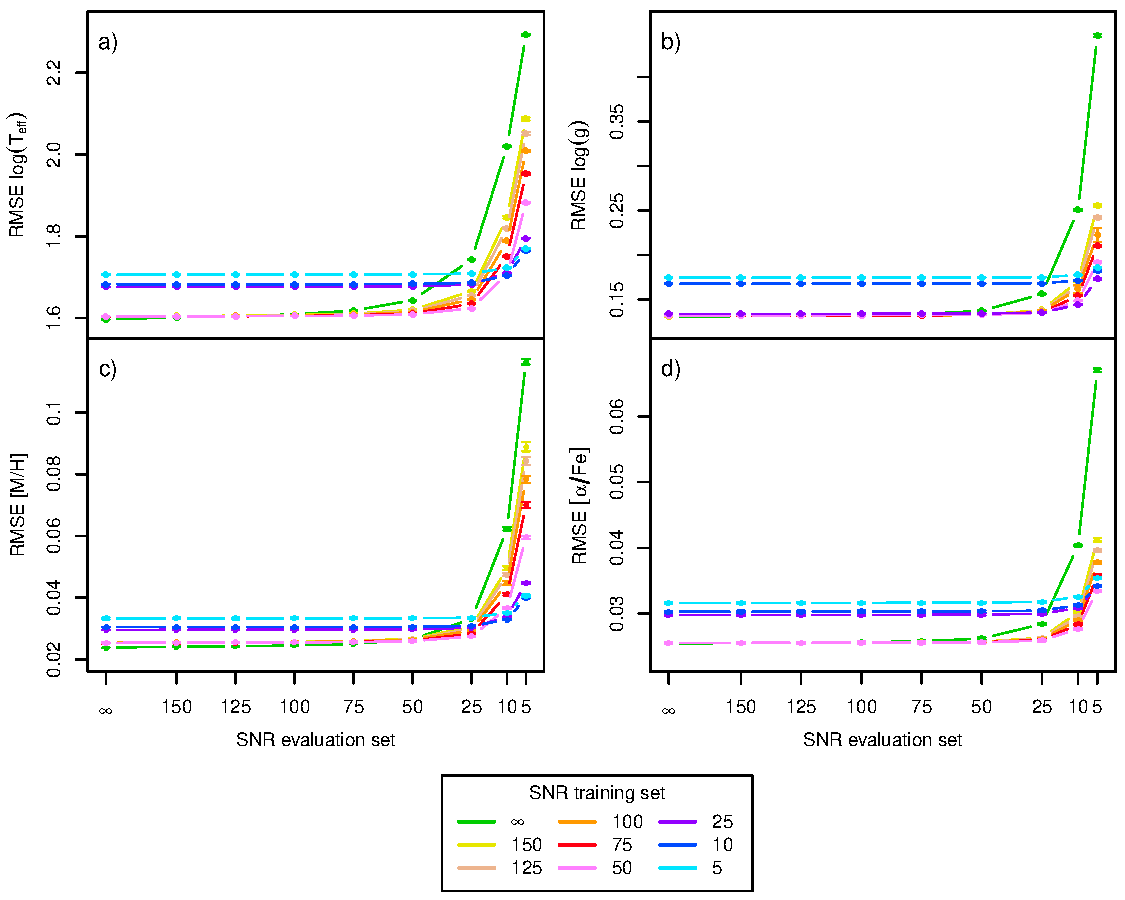
\includegraphics[width=\textwidth]{snr_errors_log_global_2x2.pdf}
\caption{Estimation errors as a function of the SNR of the evaluation
  set for $T_{\rm eff}$ (a), $\log(g)$ (b) and [M/H] (c) and
  $\left[ \alpha/Fe \right]$ (d). Each line corresponds to a model 
  trained with a specific SNR}
\label{fig:snrtrain}
\end{figure*}

As a summary, models trained with noiseless spectra are either 
catastrophic choices or just equivalent to other models. Moreover, 
there is no need to match the SNR of the training set to that of the 
real spectra because only two ICA+SVM models would be enough to 
estimate $T_{\rm eff}$ and [M/H] in all SNR regimes: the one trained 
with SNR=50 for SNR$\ge$25 and the one trained with SNR=10 for spectra 
with SNR$<$ 10. For the prediction of surface gravities, the SNR=25 model 
is sufficient for any spectrum of whatever SNR. For the prediction of 
the ratio between the alpha-elements and iron, the SNR=50 model is 
sufficient for any spectrum of whatever SNR.


%%%%%%%%%%%%%%%%%%%%%%%%%%%%%%%%%%%%%%%
\section{Training set density}
\label{sec:comparison3}

Finally, we carry out an analysis of the effect of the training set
grid density over the regression performance.  To do this, six new
grids of synthetic spectra with different grid densities were used to
train SVM models. The $T_{\rm eff}$ values varied between 4000 and
8000 K with a variable step-size between 50 K and 250 K. The other
grid parameters were established as follows: the log \textit{g} were
regularly sampled from 1 to 5 in 0.5 steps and both [M/H] and $\left[
  \alpha/Fe \right]$ were set equal to zero for
simplicity. Table~\ref{tab:grid} presents the step-sizes used in this
study as well as the number of synthetic spectra available in each
grid.  In addition to this, noisy replicates of these grids were
generated of different SNR levels (100, 50, 25, 10).

\begin{table}
\centering
\caption{Size of the new datasets computed with different grid densities.}
\label{tab:grid}
\begin{tabular}{c c}
\hline
\textbf{$T_{\rm eff}$ step-size (K)} & \textbf{Number of spectra} \\
\hline
50 & 679 \\
62.5 & 545 \\
100 & 343 \\
125 & 277 \\
200 & 175\\
250 & 143\\
\hline
\end{tabular}
\end{table}

We evaluated the performance of the SVM regression models using
10-fold cross validation. Figures \ref{fig:grid50} and
\ref{fig:grid10} presents the $T_{\rm eff}$ estimation errors obtained
with the different grid densities and the two optimal training set
SNRs (50 and 10) found in the previous Section. The main conclusions
of the analysis of these figures are the following:

\begin{itemize}
\item As expected, estimation errors increase when the grid 
	density decreases.
\item Overall, the accuracy obtained against the grid density 
	is more variable when the number of dimensions retained 
	increases. 
\item PCA and ICA show a similar behaviour with the grid density
  variation.
\item The grid density appears to have less effect over the
  performance of Wavelets and diffusion maps.
\end{itemize}

\begin{figure*}
\centering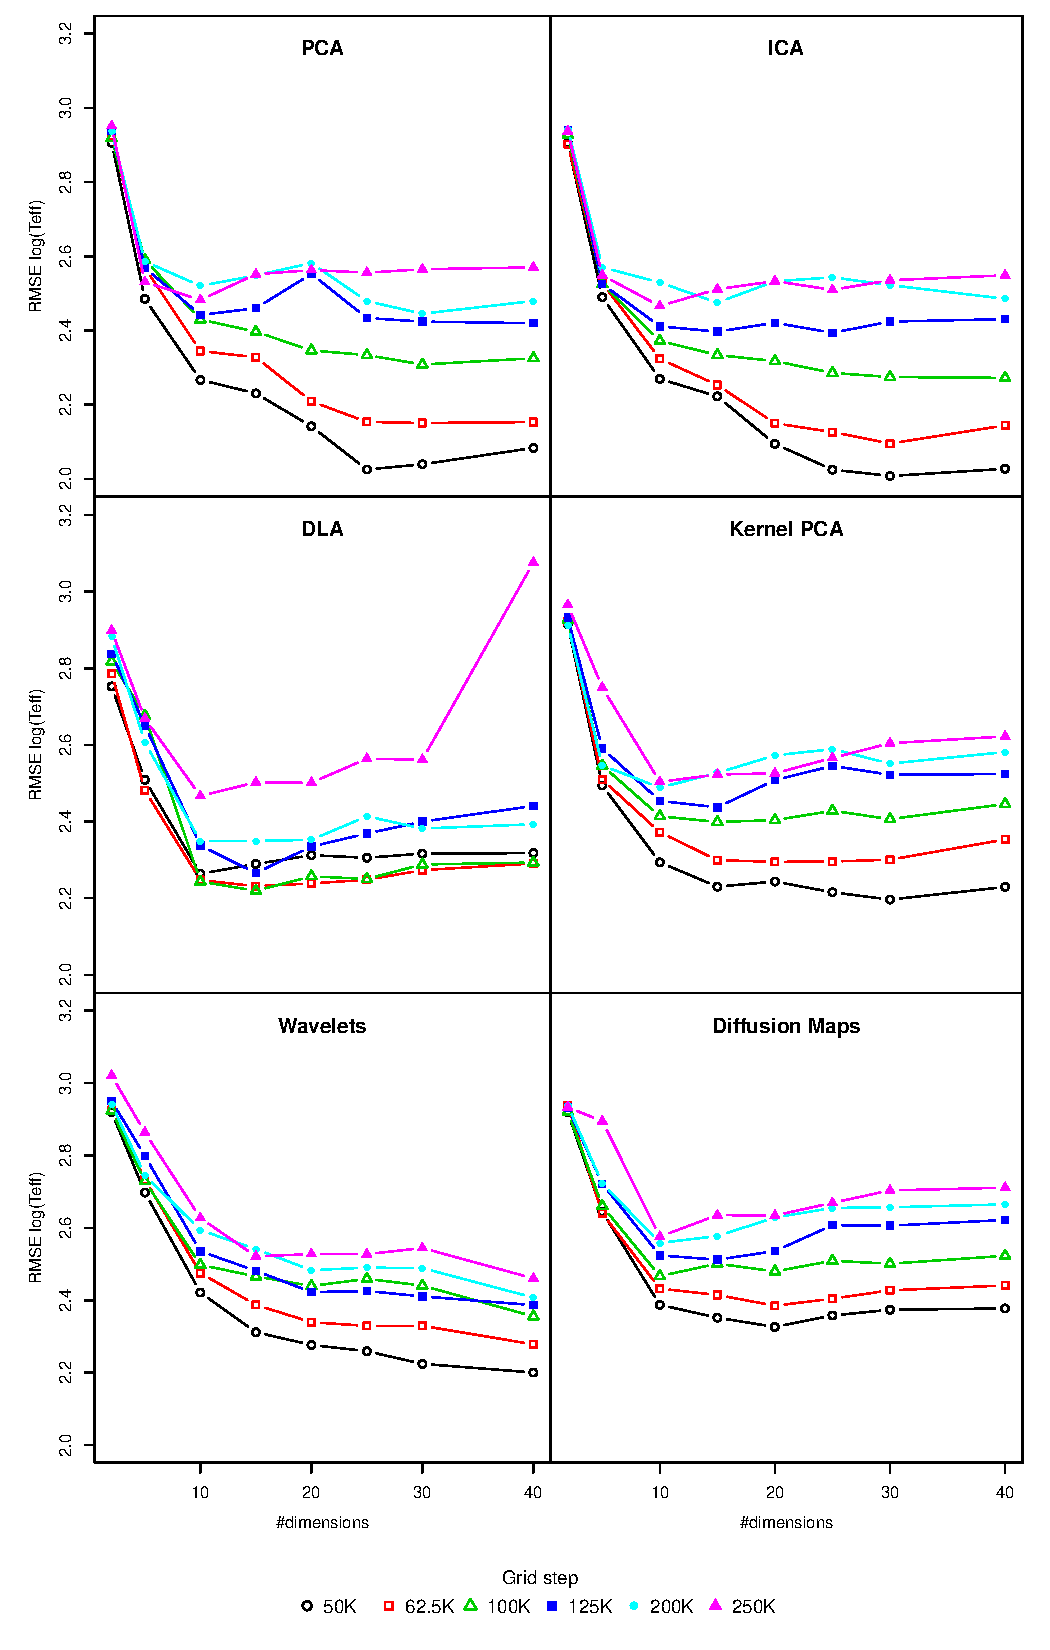
\includegraphics[height=0.95\textheight]{bestSVM_Teff_N-RMSE_HR10_snr=50_all.pdf}
\caption{Temperature estimation error against the number of dimensions
  used for data compression. Each line corresponds to a model trained
  with a specific grid step (SNR = 50)}
\label{fig:grid50}
\end{figure*}

\begin{figure*}
\centering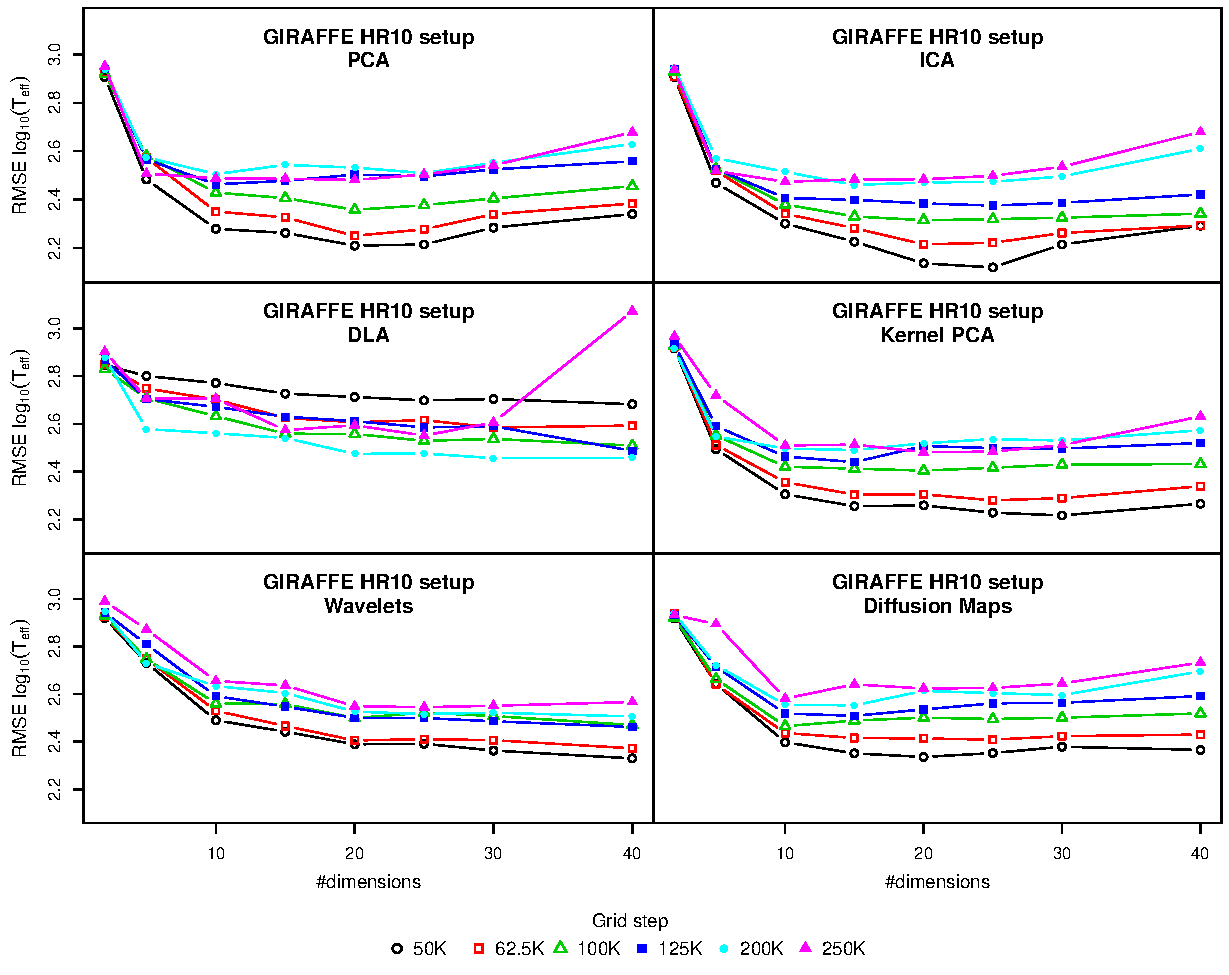
\includegraphics[height=0.95\textheight]{bestSVM_Teff_N-RMSE_HR10_snr=10_all.pdf}
\caption{Temperature estimation error against the number of dimensions
  used for data compression. Each line corresponds to a model trained
  with a specific grid step (SNR = 10)}
\label{fig:grid10}
\end{figure*}




\section{Conclusions}
\label{sec:conclusions}

{\bf Here we should discuss the validity of our conclusions. The
  validity depends on our assumptions and the experiments carried
  out. For example, they are based on SVM models with radial kernel
  functions and the implications should be stressed. Also the spectra
  were trimmed in a wavelength range: how is this range? Also compare
  our RMSE with those in the bibliography, for example, those of
  MATISSE, the Gaia-ESO results...}

{\bf Discuss the impact of including other metallicities and alpha
  abundances in the training set. To be analysed in a subsequent
  paper.}

{\bf Discuss the relationship between the methods tested here and
  those in the bibliography.}

\section*{Acknowledgements}
This research was supported by the Spanish Ministry of Economy and
Competitiveness through grant AyA2011-24052.



%%%%%%%%%%%%%%%%%%%%%%%%%%%%%%%%%%%%%%%%%%%%%%%%%%

%%%%%%%%%%%%%%%%%%%% REFERENCES %%%%%%%%%%%%%%%%%%

% The best way to enter references is to use BibTeX:

\bibliographystyle{mnras}
\bibliography{references} % if your bibtex file is called example.bib

%%%%%%%%%%%%%%%%%%%%%%%%%%%%%%%%%%%%%%%%%%%%%%%%%%

%%%%%%%%%%%%%%%%% APPENDICES %%%%%%%%%%%%%%%%%%%%%

\appendix

\section{Additional figures}
\label{app}
\begin{figure}
\centering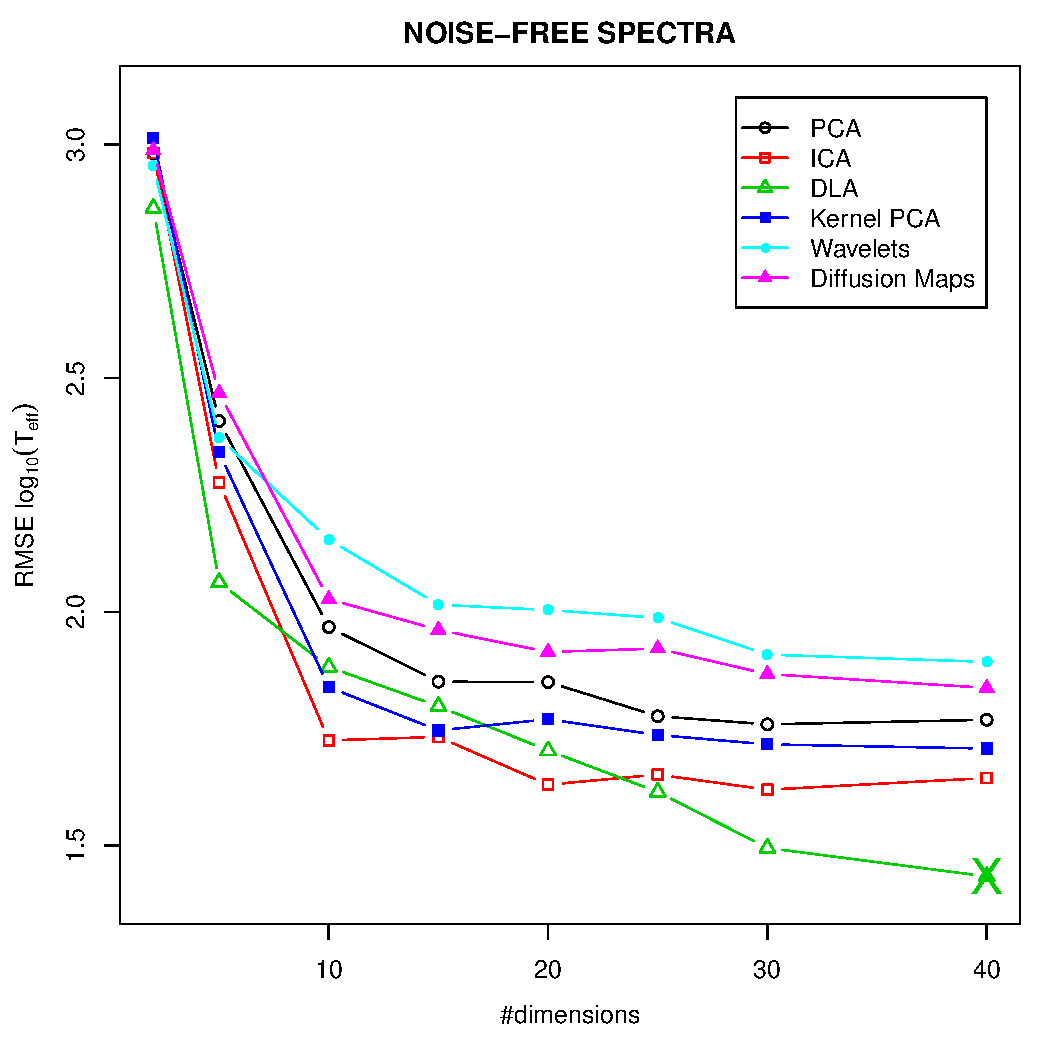
\includegraphics[width=\columnwidth]{flamesHR10_SNR=000_Teff_log_BestSVM_N-RMSE_test.pdf}
\caption{Temperature estimation error as a function of the number of
  dimensions used for data compression, for synthetic spectra}
\label{fig:01}
\end{figure}


\begin{figure}
\centering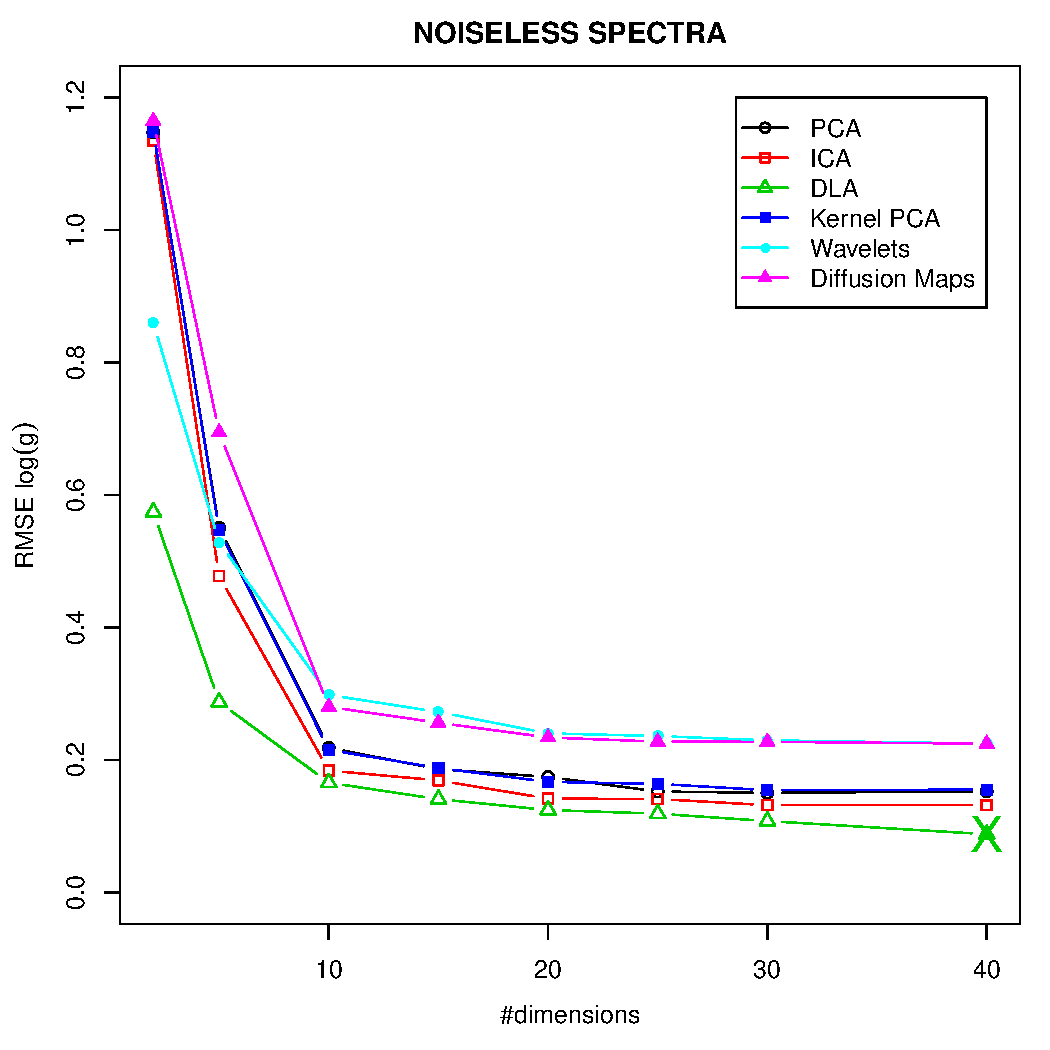
\includegraphics[width=\columnwidth]{flamesHR10_SNR=000_Logg_BestSVM_N-RMSE_test.pdf}
\caption{Surface gravity estimation error as a function of the number of
  dimensions used for data compression, for synthetic spectra}
\label{fig:03}
\end{figure}

\begin{figure}
\centering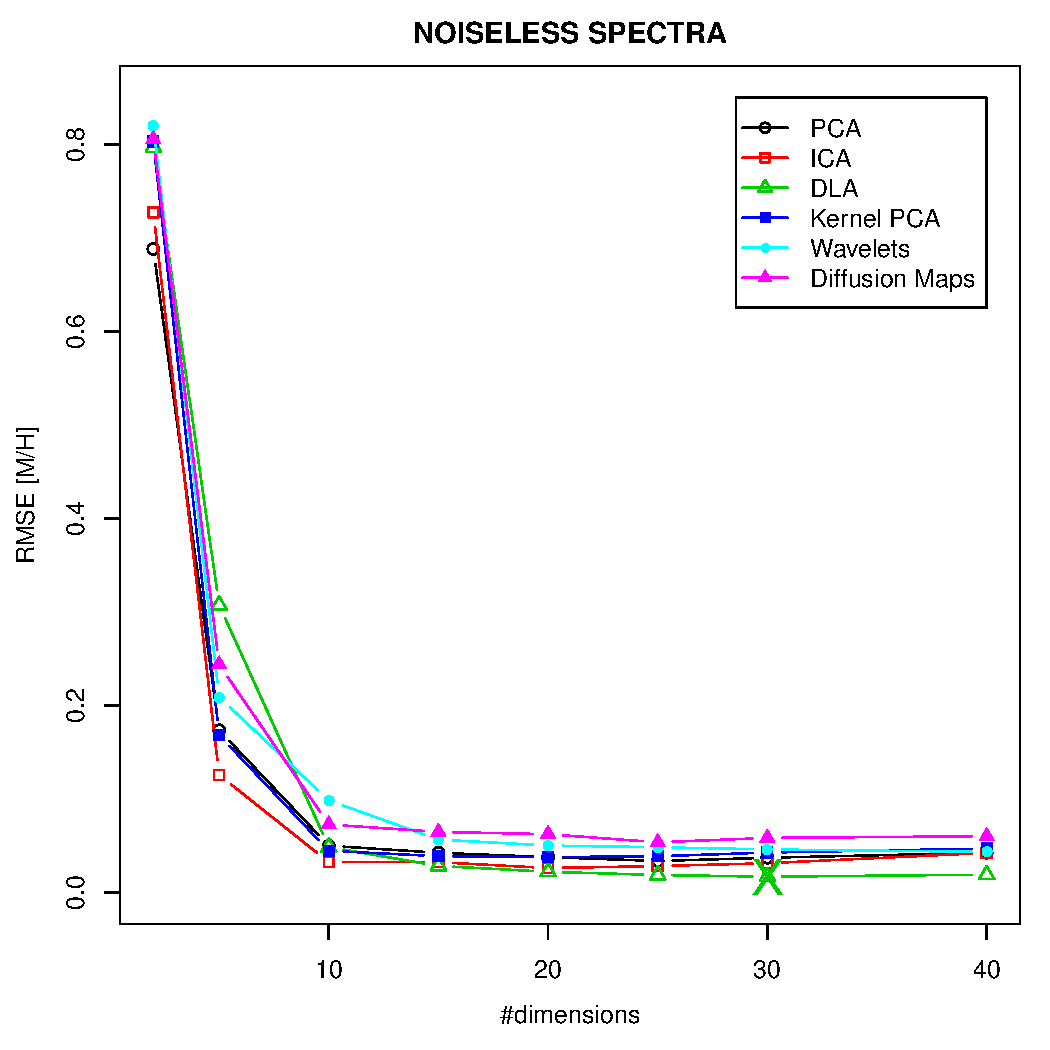
\includegraphics[width=\columnwidth]{flamesHR10_SNR=000_Meta_BestSVM_N-RMSE_test.pdf}
\caption{Metallicity estimation error as a function of the number of
  dimensions used for data compression, for synthetic spectra}
\label{fig:05}
\end{figure}

\begin{figure}
\centering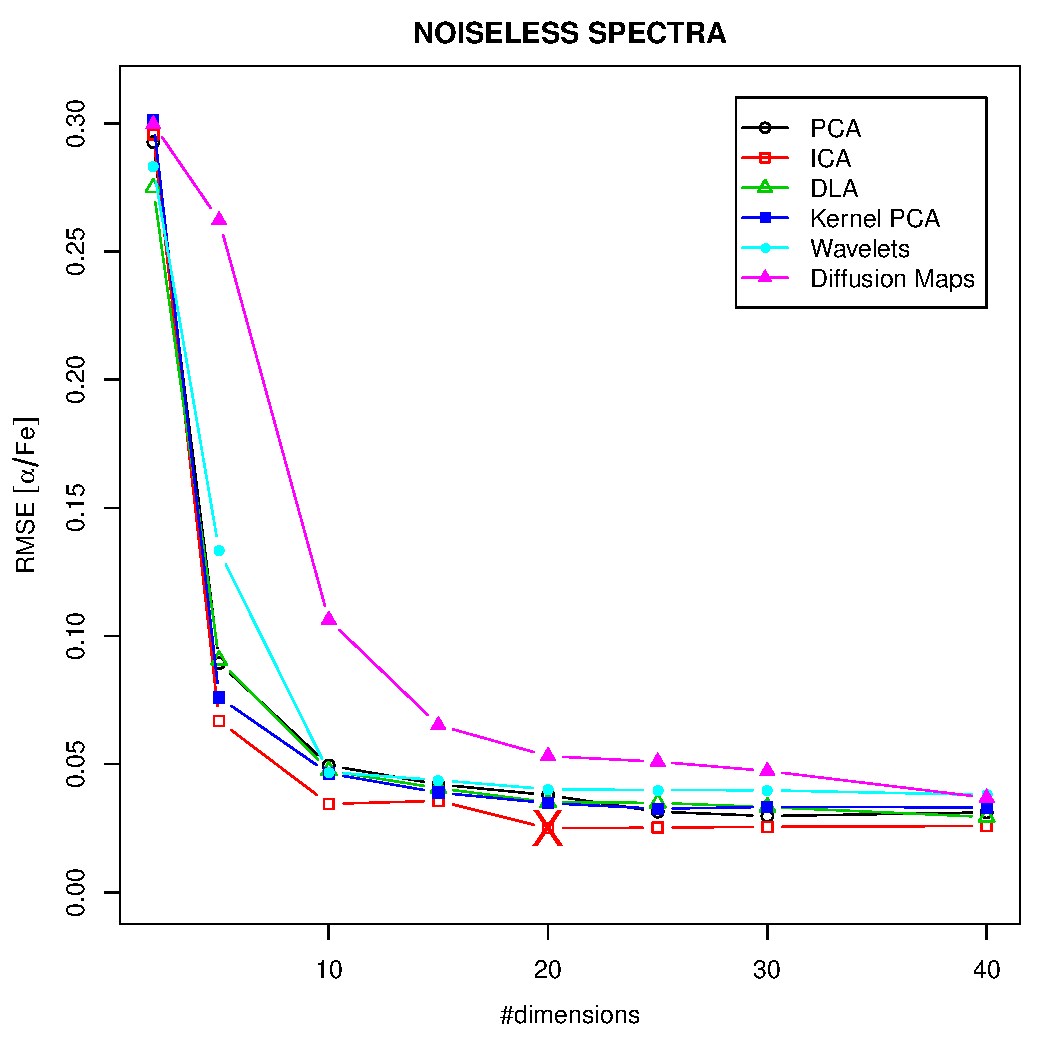
\includegraphics[width=\columnwidth]{flamesHR10_SNR=000_AlFe_BestSVM_N-RMSE_test.pdf}
\caption{$\left[  \alpha/Fe \right]$ estimation error as a function of the 
number of dimensions used for data compression, for synthetic spectra}
\label{fig:noiseless-alfe}
\end{figure}

\begin{figure*}
\centering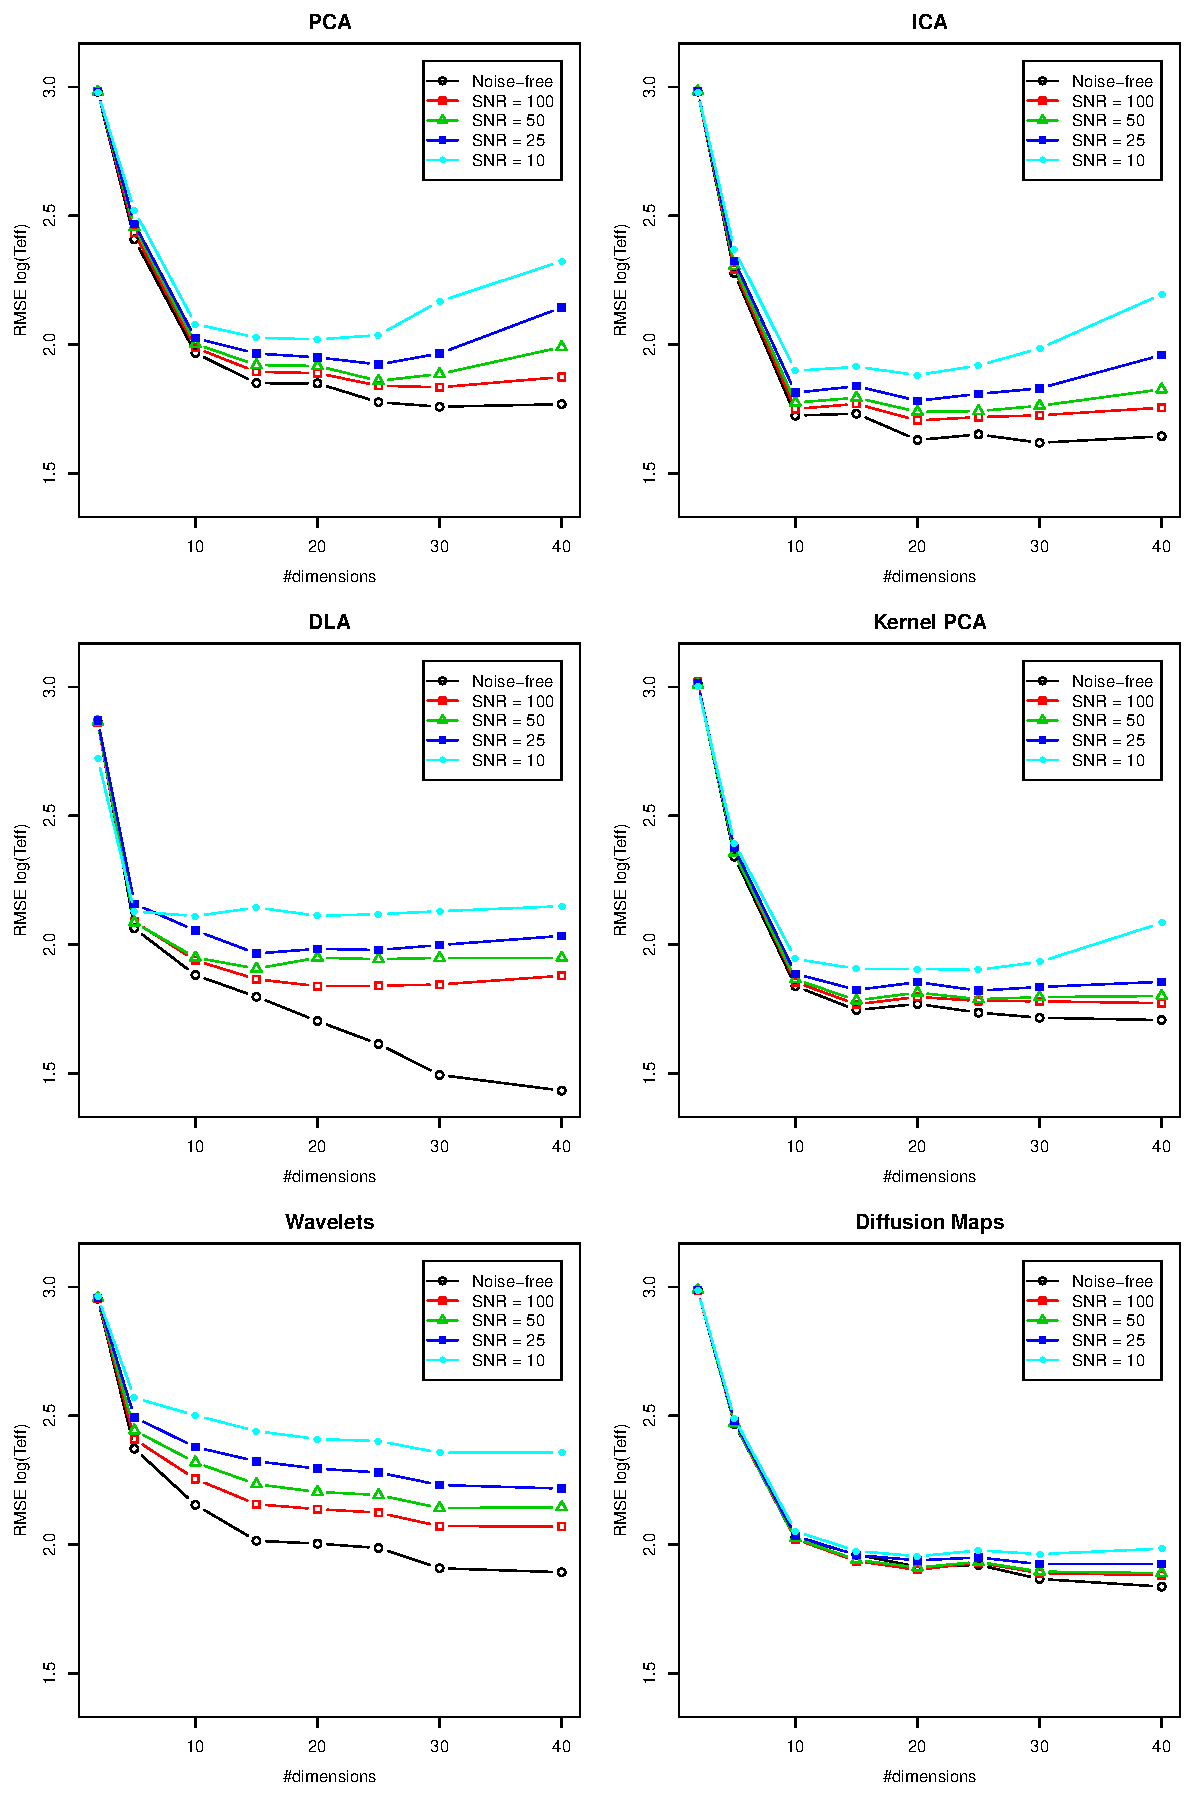
\includegraphics[height=0.95\textheight]{flamesHR10_Teff_log_BestSVM_N-SNR-RMSE_test.pdf}
\caption{Temperature estimation error against the number of dimensions
  used for data compression. Each line corresponds to a model trained
  with a specific SNR}
\label{fig:methodsnrTeff}
\end{figure*}

\begin{figure*}
\centering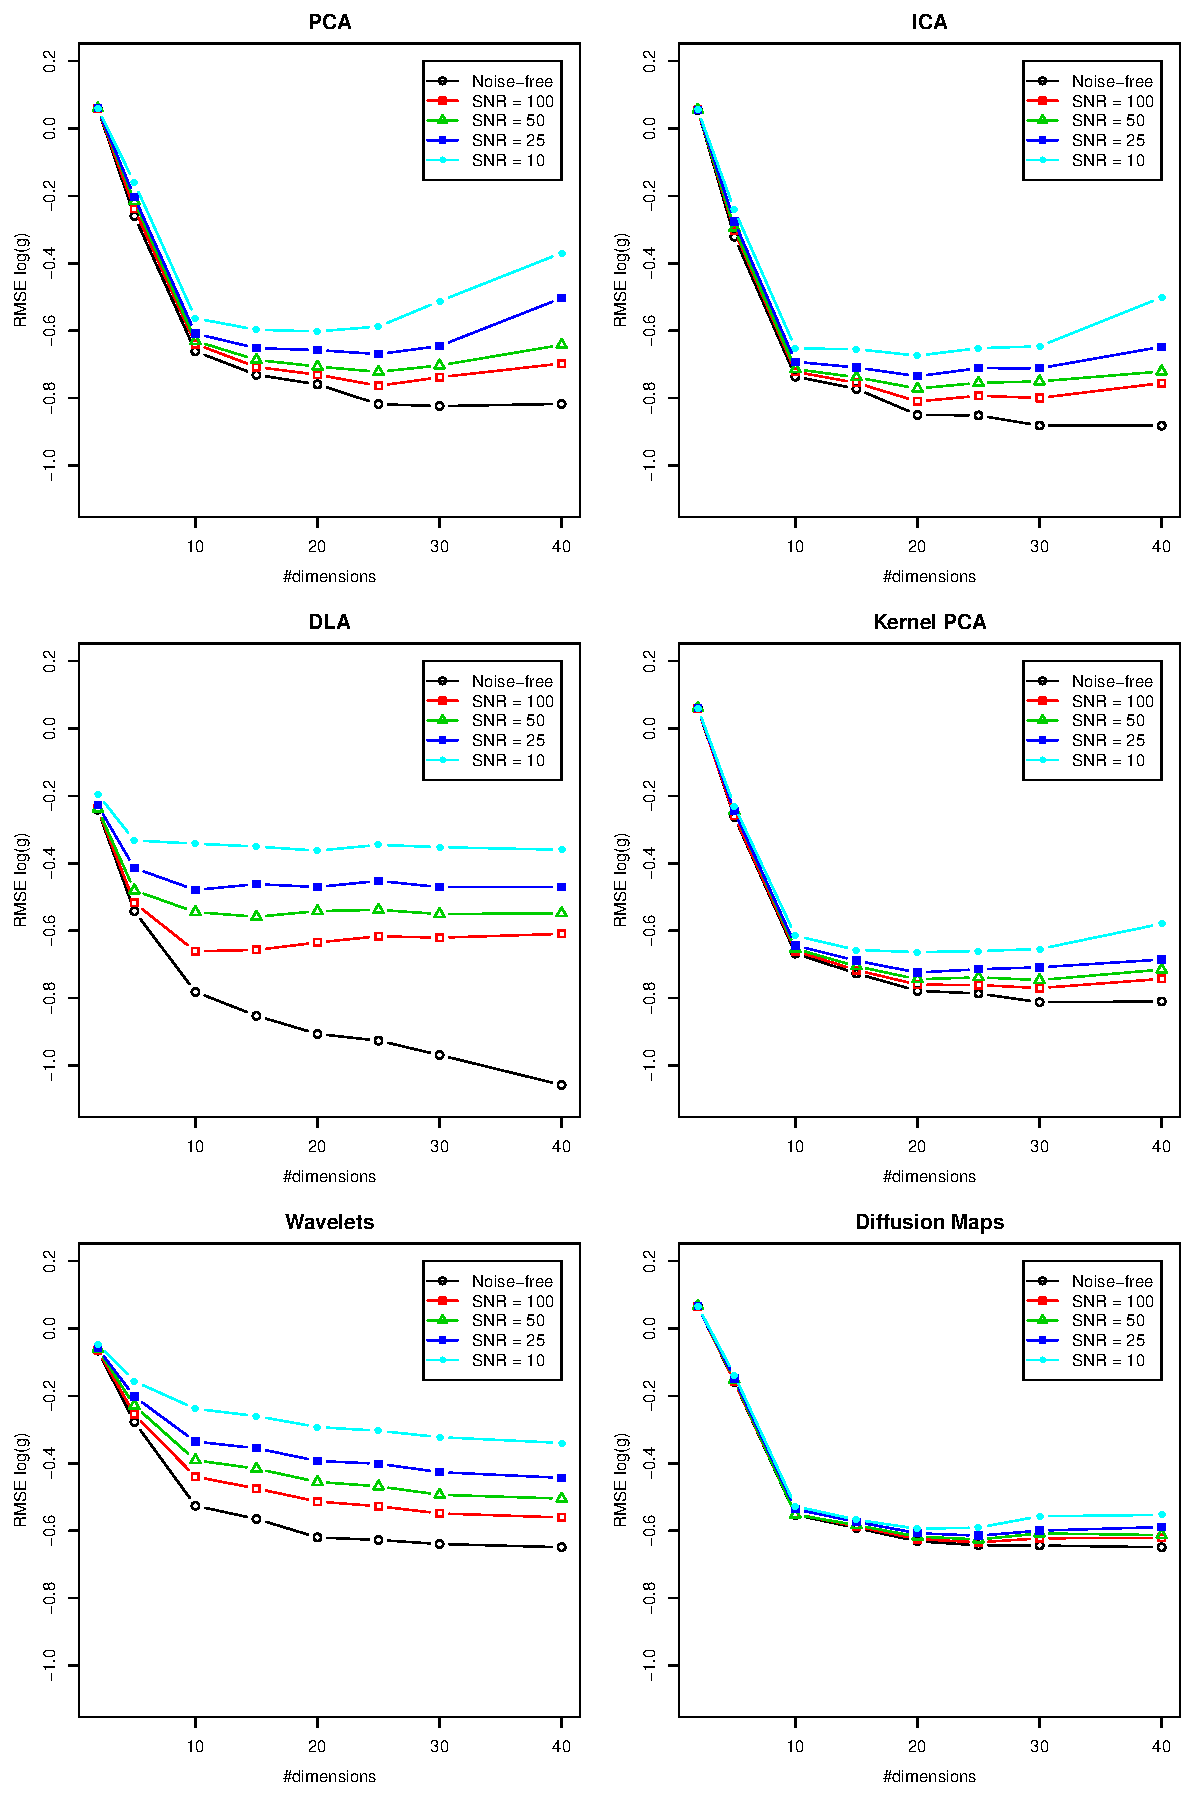
\includegraphics[height=0.95\textheight]{flamesHR10_Logg_log_BestSVM_N-SNR-RMSE_test.pdf}
\caption{Surface gravity estimation error against the number of dimensions
  used for data compression. Each line corresponds to a model trained
  with a specific SNR}
\label{fig:methodsnrLogg}
\end{figure*}

\begin{figure*}
\centering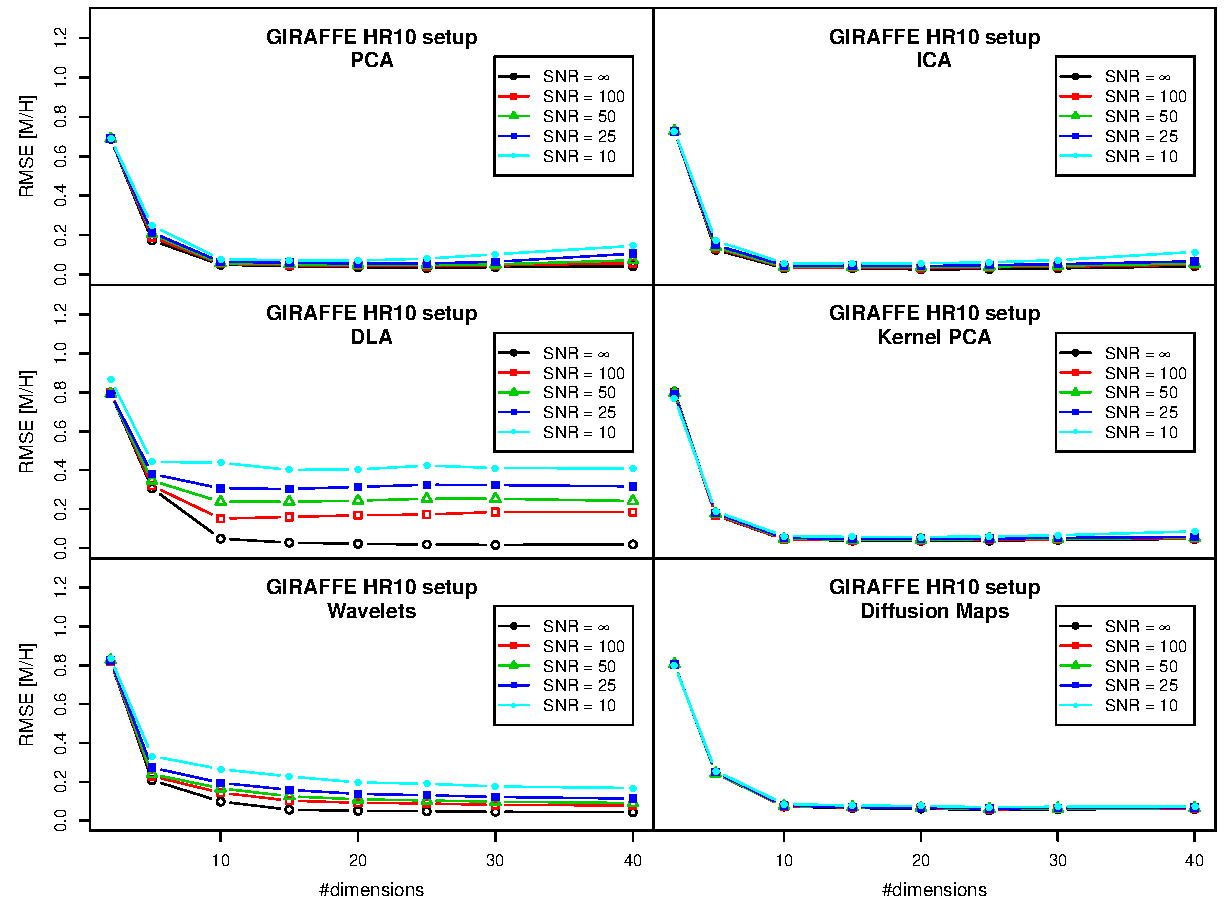
\includegraphics[height=0.95\textheight]{flamesHR10_Meta_log_BestSVM_N-SNR-RMSE_test.pdf}
\caption{Metallicity estimation error against the number of dimensions
  used for data compression. Each line corresponds to a model trained
  with a specific SNR}
\label{fig:methodsnrMeta}
\end{figure*}

\begin{figure*}
\centering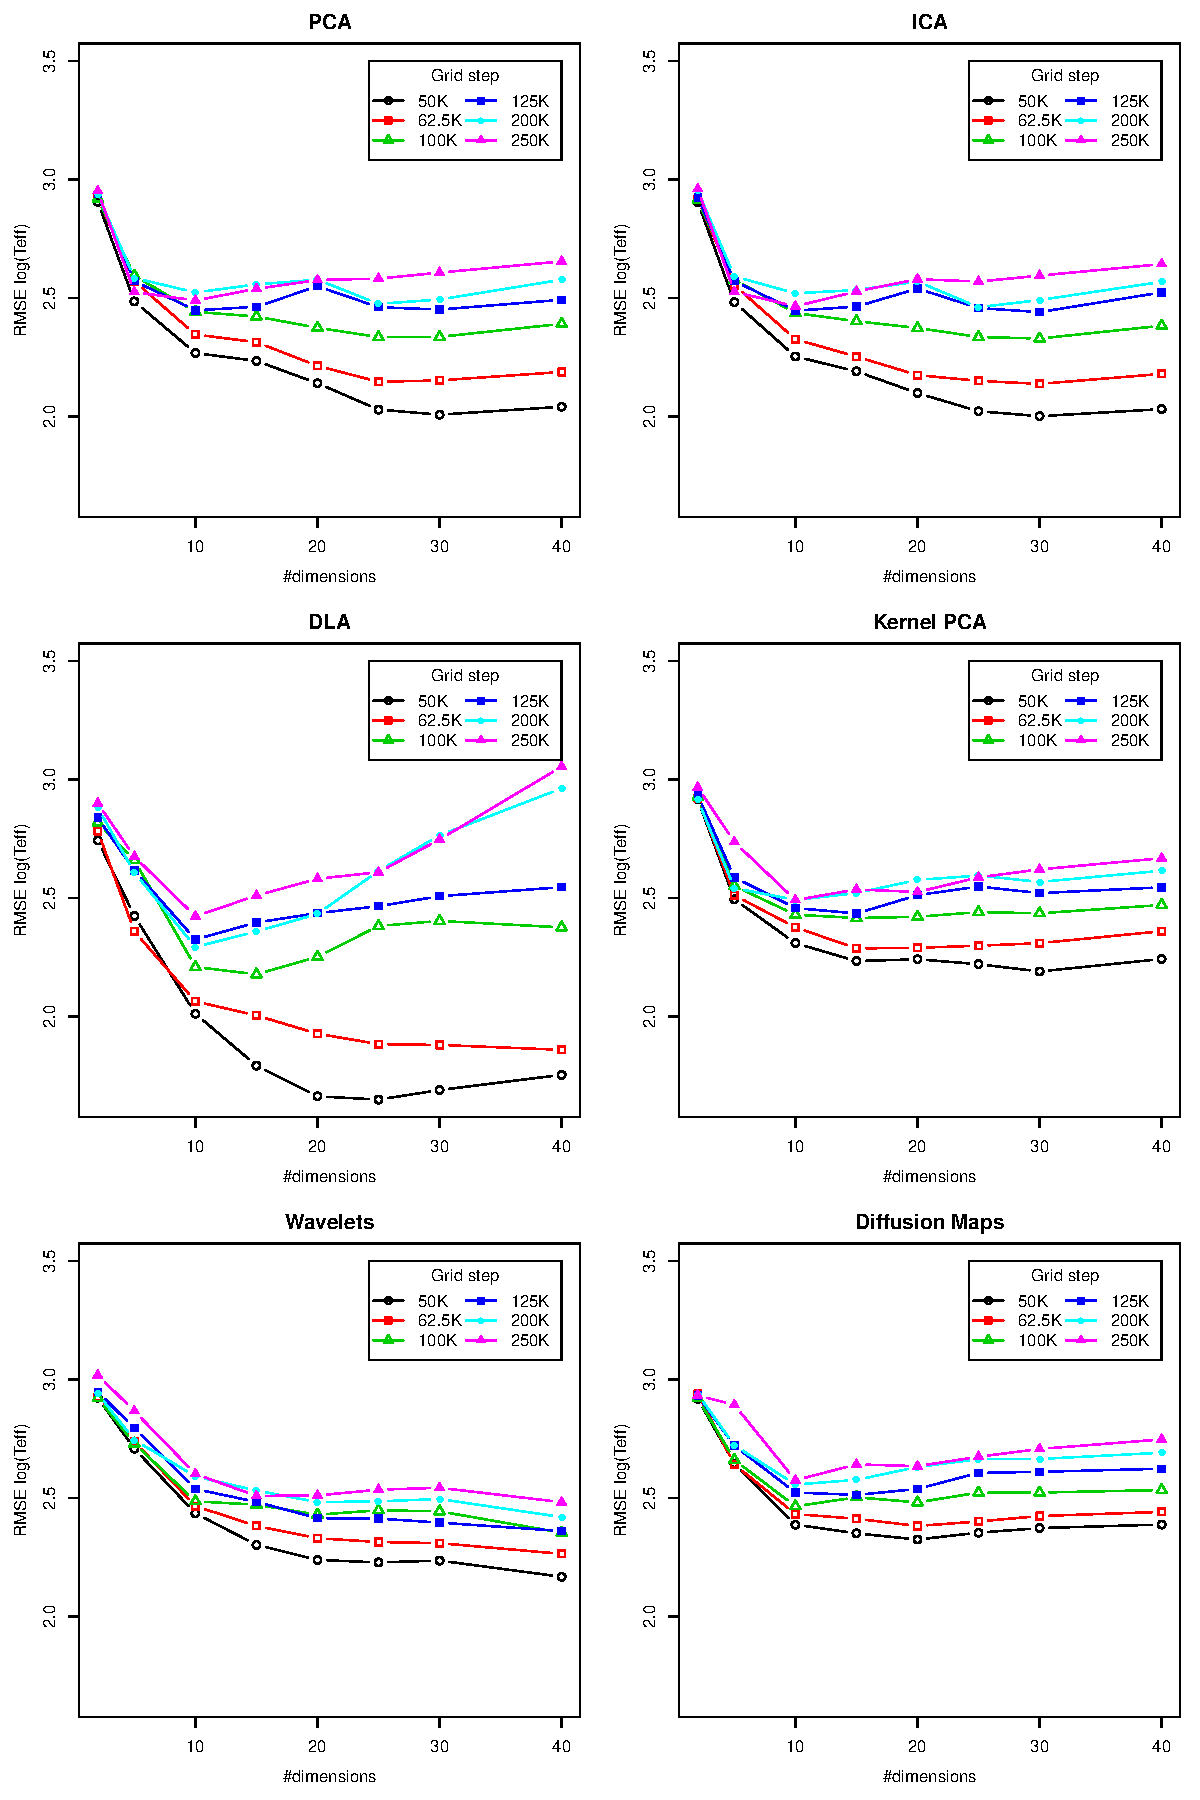
\includegraphics[height=0.95\textheight]{bestSVM_Teff_N-RMSE_HR10_pure_all.pdf}
\caption{Temperature estimation error against the number of dimensions
  used for data compression. Each line corresponds to a model trained
  with a specific grid step (Noise-free spectra)}
\label{fig:gridpure}
\end{figure*}

\begin{figure*}
\centering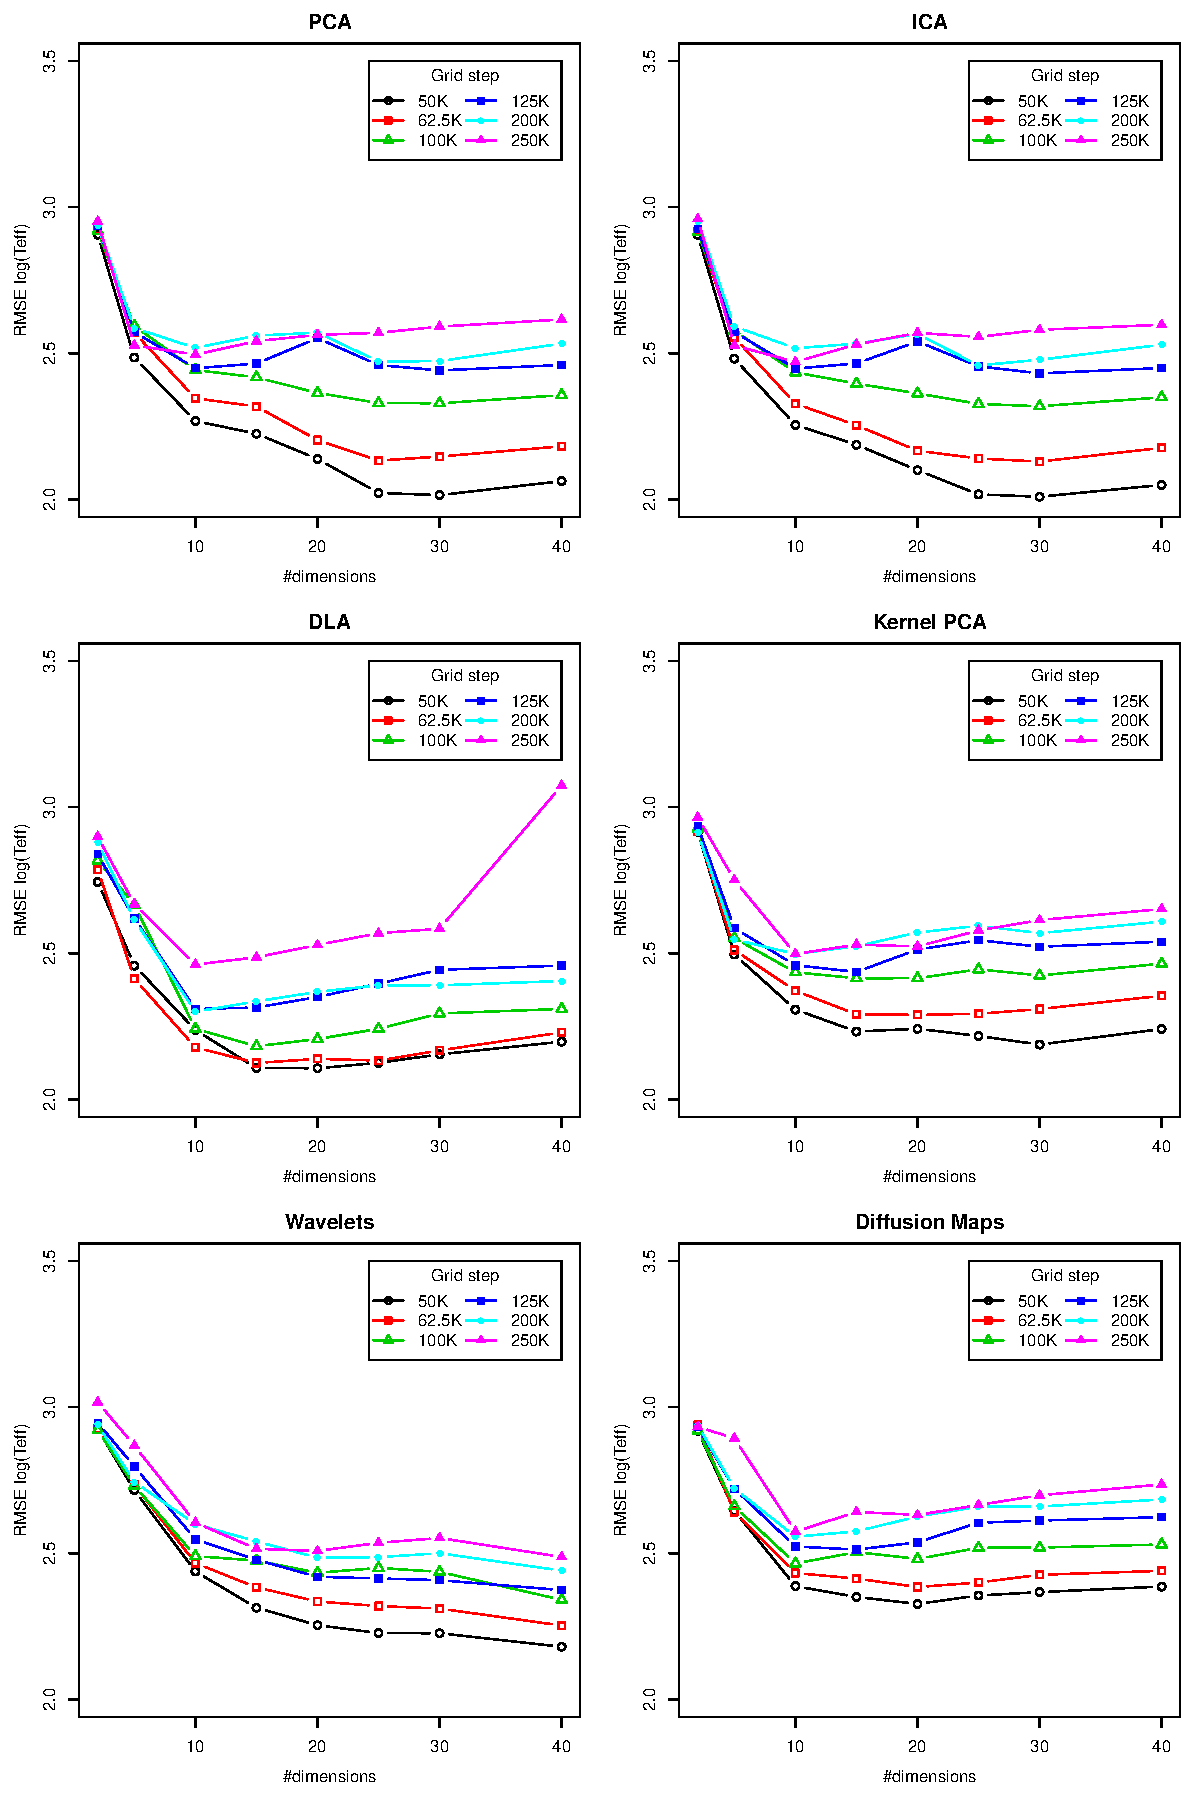
\includegraphics[height=0.95\textheight]{bestSVM_Teff_N-RMSE_HR10_snr=100_all.pdf}
\caption{Temperature estimation error against the number of dimensions
  used for data compression. Each line corresponds to a model trained
  with a specific grid step (SNR = 100)}
\label{fig:grid100}
\end{figure*}

\begin{figure*}
\centering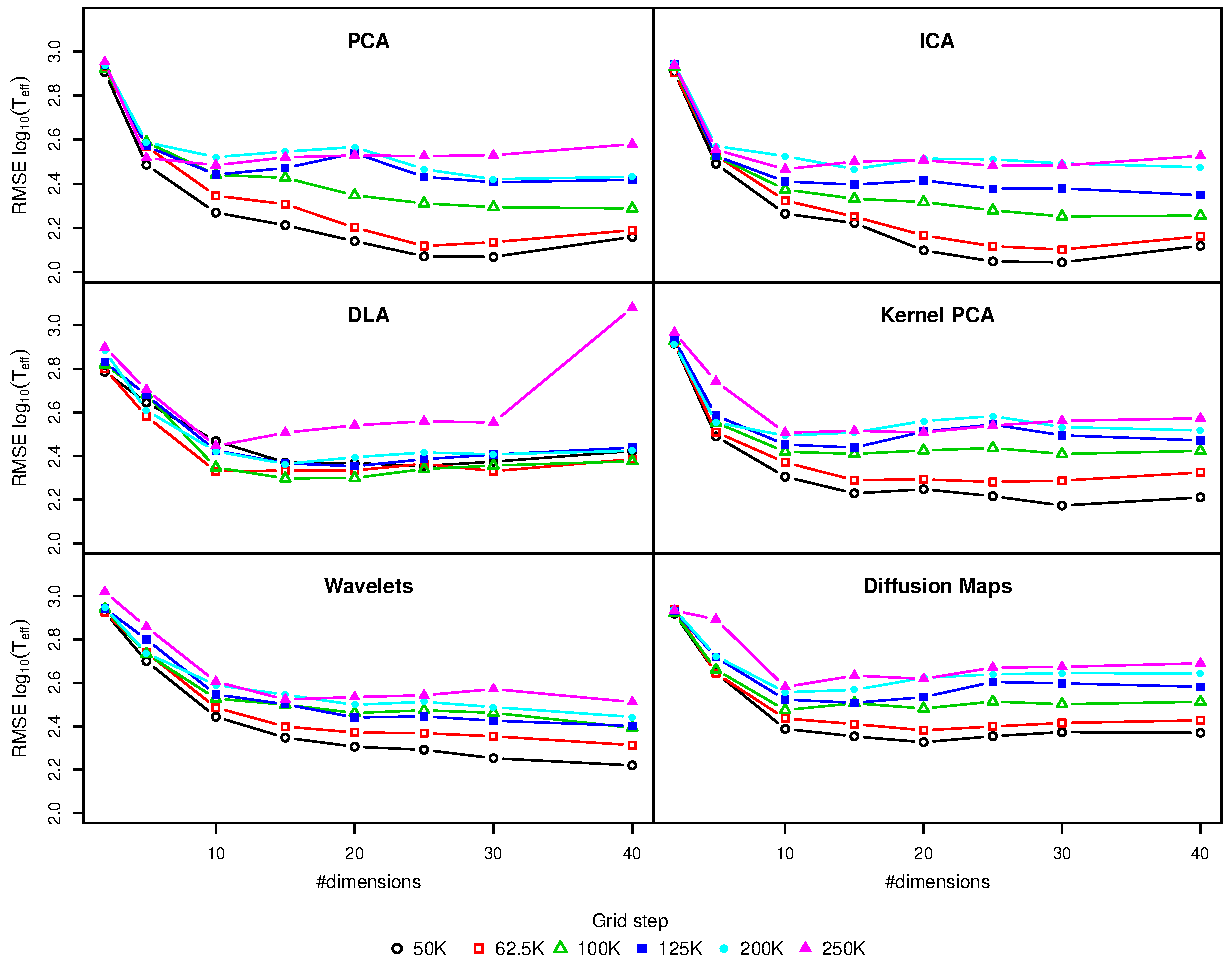
\includegraphics[height=0.95\textheight]{bestSVM_Teff_N-RMSE_HR10_snr=25_all.pdf}
\caption{Temperature estimation error against the number of dimensions
  used for data compression. Each line corresponds to a model trained
  with a specific grid step (SNR = 25)}
\label{fig:grid25}
\end{figure*}

%%%%%%%%%%%%%%%%%%%%%%%%%%%%%%%%%%%%%%%%%%%%%%%%%%


% Don't change these lines
\bsp	% typesetting comment
\label{lastpage}
\end{document}

% End of mnras_template.tex
